\documentclass[a4paper,12pt, final]{report}
\usepackage{graphicx}
\graphicspath{{./}{./fig/}}
\usepackage{url}
%\usepackage[nomain,acronym,xindy,toc]{glossaries} % nomain, if you define glossaries in a file, and you use \include{INP-00-glossary}
%\makeglossaries
%\usepackage[xindy]{imakeidx}
%\makeindex
%\usepackage[section]{placeins}
\renewcommand\bibname{References}
\usepackage[utf8]{inputenc}
%\usepackage{algorithm2e}
%\usepackage{wrapfig}
\usepackage{epsfig}
%\usepackage{hyperref}
\usepackage[hidelinks]{hyperref} % To Hide the box around links
\renewcommand\bibname{References}
%\usepackage{algorithm2e}
\usepackage{color}
\usepackage{textcomp}
\usepackage{acronym}
\usepackage{mathtools}
\usepackage{amsmath}
\usepackage[top=0.5in, bottom=1in, left=1in, right=1in]{geometry}
\geometry{verbose,tmargin=3cm,bmargin=3cm,lmargin=2.8cm,rmargin=2.8cm}
\usepackage{xcolor}
\usepackage{comment}
\usepackage{fancyvrb,fvextra}
\usepackage{booktabs}
\usepackage{array}
\usepackage{algpseudocode}
\usepackage{algorithm}
\usepackage{algorithmicx}

\newcolumntype{P}[1]{>{\centering\arraybackslash}p{#1}}

\definecolor{dark-red}{rgb}{0.4,0.15,0.15}
\definecolor{dark-blue}{rgb}{0.15,0.15,0.4}
\definecolor{medium-blue}{rgb}{0,0,0.5}

\fvset{tabsize=2}

\newcommand{\BigO}[1]{\ensuremath{\operatorname{O}\bigl(#1\bigr)}}
\parindent 8pt
\begin{document}
  \thispagestyle{empty}
  \vspace*{0.9cm}
  {\centering     
  \textbf{\LARGE An AI/ML Inference Engine Developed Using AHIR-V2 Tools}\\
  \vspace{1.10cm}
  %\it
  %\vspace{.5cm}
  %\rm
  \textbf{\large Dual Degree Project Report}\\
  \vspace{0.7cm}
  {Submitted in partial fulfilment of the requirements}\\
  \vspace{0.25cm}
  {for}\\
  \vspace{0.9cm}
  \textbf{ Dual Degree (B.Tech + M.Tech)\\ in Electrical Engineering \\with specialization in Electronic Systems}\\
  \vspace{1.00cm}
  {by}\\
  \vspace{0.20cm}
  \textbf{\large Aman Dhammani}\\
  \vspace{0.25cm}
  \textbf{\large (Roll No. 18D180002)}\\
  \vspace{1.7cm}
    \begin{figure}[htb]
    \begin{center}
    
\includegraphics[height=1.5in,width=1.5in]{iitblogo.png}
    \end{center}
    \end{figure}
  \vspace{1.350cm}
  {Under the supervision of}\\
  \vspace{0.20cm}
  \textbf{\large Prof. Madhav P. Desai}\\
    \vspace{0.30cm}

    
  {\textbf{Department of Electrical Engineering}}\\
  {\textbf{Indian Institute of Technology Bombay}}\\
  {\textbf{2023}}
 
 }

\newpage

\chapter*{}
\begin{center}
{\Large \textbf{Dissertation Approval}}

\bigskip
\bigskip
\bigskip
This dissertation entitled\\
\bigskip
\textbf{An AI/ML Inference Engine Developed Using AHIR-V2 Tools}\\
\bigskip

by\\
\bigskip

Aman Dhammani\\
Roll No. 18D180002\\
\bigskip
is approved for the degree of\\
\textbf{B.Tech + M.Tech in Electrical Engineering}\\

\end{center}
 \vspace{10mm}
\begingroup
\setlength{\tabcolsep}{30pt}
\begin{center}
    \begin{tabular}{c c}
        ..................................................... & .....................................................\\
        Prof. Madhav P. Desai & Prof. D. Manjunath\\
        (Supervisor)     & (Examiner)\\
        \\\\
        ..................................................... & .....................................................\\
        Prof. Kavi Arya   & Prof. Kavi Arya\\
        (Chairperson) & (Examiner)\\
    \end{tabular}
\end{center}
\endgroup
\bigskip
{Date: June 30, 2023}\\
{Place: IIT Bombay}


  \thispagestyle{empty}

% ------------------------------------------------------------------------------
\newpage
 \linespread{1.5}
\chapter*{Declaration}
%\pagenumbering{gobble}
I declare that this written submission represents my ideas in my own words and where others ideas or words have been included, I have adequately cited and referenced the original sources.
\newline
\newline
I also declare that I have adhered to all principles of academic honesty and integrity and have not misrepresented or fabricated or falsified any idea/data/fact/source in my submission. I understand that any violation of the above will be cause for disciplinary action by the Institute and can also evoke penal action from the sources which have thus not been  properly cited or from whom proper permission has not been taken when needed.

\vspace{3.0cm}
\begin{flushright}
\line(1,0){140}\\
\vspace*{10pt}
\textbf{Aman Dhammani} \\
\textbf{Roll No. 18D180002} \\
IIT BOMBAY
\end{flushright}
\begin{flushleft}
Date: June 30, 2023
%\line(1,0){75}
\end{flushleft}

  \thispagestyle{empty}
\newpage

\renewcommand{\abstractname}{Acknowledgement}
\begin{abstract}
I express my heartfelt gratitude to my guide Prof. Madhav Desai for providing me the opportunity to work on this topic and for his valuable guidance throughout the project. His advice has helped me in gaining a better understanding of the research topic.\\\\
I would also like to thank Harshad Ugale for his collaboration in the development and validation of the System On Chip.\\\\
\\\\
\\\\
\\\\
Aman Dhammani\\
Electrical Engineering\\
IIT Bombay\\\

\end{abstract}

  \thispagestyle{empty}

\newpage 
\pagenumbering{roman}
\renewcommand{\abstractname}{Abstract} 
\abstract{
	Convolutional Neural Networks form a major part of today's image processing tasks. The continual rise in depth of such networks, coupled with larger intermediate feature maps leads to a requirement of computation in the order of billions of MACs (Multiply and Accumulate) for processing each image. At the same time, such huge tensor sizes and limited memory bandwidth prevent storing of all data on small on-chip buffers. This calls for the need of accelerators with a large number of processing elements designed for efficient reuse the data.

We present a high-performance input-streaming based CNN inference engine operating with small buffer sizes and designed using AHIR-V2, a high level synthesis framework. Using the given design, we demonstrate an end-to-end image segmentation pipeline on a commercially available FPGA, achieving an average performance of over 83 Gigaoperations per second (GOPS) when run at a clock frequency of 125MHz. During the execution, we exhibit a peak performance of 96 GOPS with 100\% compute resource utilisation with a compute-to-memory ratio of over 873 operations/byte indicating high data reuse.

We also integrate a cluster of eight engines with a 32-bit AJIT processor and a Network Interface Controller to generate an SoC achieving an average throughput of over 300 GOPS and image throughput of 5 fps. Using these results, we show that the performance per resource of our engine is competitive with those of the implementations reported in literature.
}

\tableofcontents
  %\addcontentsline{toc}{chapter}{\listfigurename}
  %\addcontentsline{toc}{chapter}{\listtablename}
  \listoffigures
  \listoftables
%  \printglossaries

%\newglossaryentry{ILP}
%{name = ILP,
%description = Instruction Level Parallelism}


\chapter{Introduction}\label{Chap:1}
  \pagenumbering{arabic}
  \thispagestyle{empty}

Machine Learning is a thriving area in the field of Artificial Intelligence, which involves design and deployment of algorithms that can learn and predict through models trained using given datasets. In recent years, many machine learning techniques, such as Convolution Neural Networks (CNN) \cite{CNNs} and Support Vector Machines (SVM) \cite{SVMs}, have shown promise in many application domains, such as image processing and speech recognition \cite{LeNet,CNN1,GoogleNet,ALexNet,ResNet,YOLO,CNN7,CNN5}.  


We focus our attention to CNNs, which forms the backbone for most image processing tasks. They are able to capture the image data and modify them through a series of trained filters (kernels) \cite{CNNs}. However, with the increasing depth and complexities of the CNNs, accompanied by large feature maps, it leads to an enormous amounts of computation to process one image, which is beyond the capability of a CPU, which has limited avenes for data-level parallelism. Furthermore, limited on-chip memory necessitates the reuse of the data to reduce memory accesses, requiring specialised architecture with high memory bandwidths and data buffers that can leverage the high levels of parallelism available in such tasks.


Many hardware technologies are available for accelerating machine learning algorithms, which include Graphics Processing Unit (GPU), Field-Programmable Gate Array (FPGA) and Application Specific Integrated Circuits (ASIC). GPUs exploit data-level parallelism to get high performance. Nonetheless, due to its general-purpose nature, it has immense complexity, leading to high power consumption of over 200 W, and hence, is not suitable for embedded applications.


This makes FPGAs and ASICs a promising technology due to their low power consumption, reconfigurability, and real-time processing capability. However, ASICs incur high development cost and therefore, cannot be used for prototyping, making FPGAs the preferred option for development of low-cost ML accelerators \cite{FPGA1,FPGA2,FPGA3}.


\section{Design Methodology}

The system is designed using C and Aa, a hardware intermediate language \cite{ahir} capable of describing high-performance digital systems using algorithmic description. We use the AHIR-V2 toolchain \cite{ahir} for converting modules designed primarily using Aa to generate the VHDL model of the system. At the same time, the tools produce a couple of binaries using the C testbench written by the user. These testbench binaries can be used to simulate and verify the working of the C model of the hardware, and the generated VHDL design, thereby allowing functional verification before hardware synthesis. The use of algorithmic design and simulation-based verification cuts down the design and verification time significantly as a majority of the functionality in the individual components can be verified and corrected before synthesising the hardware.


The generated design is then instantiated in a top-level VHDL module, which contains other peripheral modules like UART connections, DRAM controller, clock circuitry etc. Appropriate constraint files are set to provide IO functionality for the FPGA card. We use Xilinx Vivado 2019.1 to synthesize, optimise, place and route the system so that it can be deployed on VCU128 FPGA.


Use of the above EDA tools allows the programmers to focus on the algorithmic design of the system, which is then processed to give the most optimal configuration. This helps in cutting down the design and verification time, while simultaneously reducing the code size and complexity, leading to faster and easier debugging \cite{FPGA1,FPGA3}. Furthermore, due to implementation of features like pipelining and parallelization, the tools can generate low-level structures having full-rate performance.


\section{Goals}

In this thesis, we achieve the following goals:

\begin{itemize}

	\item {\bf Development and optimization} a high-performance resource-efficient AI/ML inference engine. The design was done entirely using algorithmic hardware techniques using AHIR-V2 toolchain, and, is fully functional and exhibits competitive performance relative to reported work.
	\item {\bf Incorporation and validation} of the accelerator engine on an AJIT-processor based system on chip (SoC) running on VCU128 FPGA card through an end-to-end image analysis using UNET.
	\item {\bf Demonstratation} of the scalability of the accelerator and the characterization of the speedup obtained
\end{itemize}


\section{Notations Used}

We use the following notation scheme to describe the tensors for any given operation. Subscripts \verb|i|,\verb|o|,\verb|k| are used to denote input, output and kernel respectively. We use r, c and chl to represent the parameters row, column and channel for each tensor.


Also, we use Octave/MATLAB style pseudocode, with loops and conditions of the form for...do...endfor or if...then...else...endif . Furthermore, the arrays can be multi-dimensional with A[d1start:d1end,d2start:d2end,...] denoting index d1start to d1end of dimension 1 of A, index d2start to d2end of dimension 2 of A and so on, all mentioned indices included. All indexing starts from 1. The array iteration can have steps as well, which will be represented in the form start:step:stop, both start and stop included.


\chapter{Neural Network Architecture Details}\label{Chap:2}

There are various CNN architectures used globally for various tasks, like Inception-Net \cite{GoogleNet}, ResNets \cite{ResNet},  etc. To develop and characterize our inference engine, we choose UNET as the base architecture. UNET is an CNN-based architecture proposed by Ronneberger et al. for image segmentation\cite{UNET}. It has been widely used for segmentation tasks, and provides an end-to-end image computation involving several operations used in machine learning, like convolution, padding, maxpooling, upsampling, skip connections, ReLU and sigmoid activations, making it an ideal candidate to deploy on our accelerator. We first describe the UNET architecture, and then the individual operations being used to implement the architecture.


\begin{figure}[h!]
    \centering
    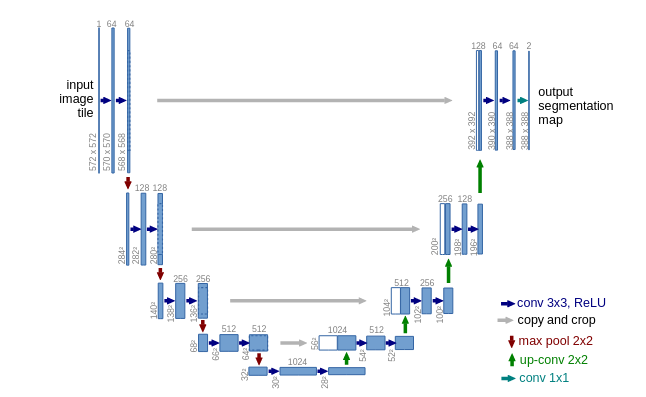
\includegraphics[width=\textwidth]{Screenshot from 2022-10-12 10-40-59.png}
	\caption{Original UNET Architectre (Image Source \cite{UNET})}
    \label{fig:UNET}
\end{figure}

The UNET architecture consists of an encoder loop, which will progressively extract the critical information from the image, creating smaller and deeper feature maps. The encoder loop extracts information by performing a series of convolution operation and maxpooling. The pooling layer helps in reducing the dimensions of the feature maps, helping in encapsulating more and more key features with fewer parameters. The convolution operations are all followed by ReLU activation to maintain non-linerity. There are four encoder loops comprising of two convolutions and a maxpooling layer each. Furthermore, the inputs of the maxpooling layer are stored to be passed on to future layers through skip connections. The left half of Figure~\ref{fig:UNET} forms the encoder network.


After the encoding is done, there are a couple of convolution operations to generate the base layer for the decoder. The decoder is designed symmetric to the encoder network. Instead of using pooling layers to downsample the image, it uses transpose convolution (see up-conv in Figure~\ref{fig:UNET} operation to upsamples the images to reconstruct the original image with the segmentation data. The grey arrows represent the skip connections from the encoder loops, which help in preserving context identified by the encoder loop. The last convolution reconstructs an image with the same dimensions as the input, giving the segmentation map based on the task at hand.



\section{Convolution}

Convolution operations are extensively used for image processing tasks. Convolution involves sliding the kernel window over the feature map and perform a dot product of the elements covered by the moving window. The tensors are assumed to be 3-dimensional with a dimension each for row, column and channel. The moving window traverses along the rows and columns, and has the same number of channels as the feature maps (input tensor).


We provide the computational expense of convolution by calculating the number of multiplications (which is the primary compute operation in convolution). Assuming same padding (i.e. input is padded such that output is as large as input), we have $r_o = r_i, c_o = c_i, chl_i = chl_k $ (default). Thus, for a kernel of size $r_k * c_k$, the number of computations to get one output element is $r_k * c_k * chl_k$ = $r_k * c_k * chl_i$. Furthermore, there are $r_o * c_o * chl_o$ such outputs.

This gives the total number of computations for one convolution layer as
\begin{equation*}
r_o * c_o * chl_o * r_k * c_k * chl_i
\end{equation*}

For a typical feature map of size 112*112*128, with 128 output channels and 3*3 kernel, this corresponds to a total over 1.8 billion multiplications for a single layer. As we have seen in Figure~\ref{fig:UNET}, the architecture involves over 18 convolution layers, leading to a computational expense of over 30 billion MAC operations.

We also provide a mathematical description for the convolution operation. A n$\times$n ($\implies r_k = c_k = n$) convolution operation can be defined as:

\begin{equation}\label{eq:conv}
	output[r,c,chl] = input[r:r+n-1,c:c+n-1,1:chl_i] \cdot kernel[chl,1:n,1:n,1:chl_i]
\end{equation}
where $\cdot$ denotes the dot product between two tensors.


Using Equation~\ref{eq:conv}, the algorithm for convolution is described in Algorithm~\ref{Algo:conv}.


\begin{algorithm}
	\caption{Pseudocode for computation of convolution}
	\label{Algo:conv}
	\begin{algorithmic}[1]
\For {co = 1:chl\_o}
	\For {r = 1:r\_o}
		\For {c = 1:c\_o}
			\State $tmp \gets 0$
			\For {r' = 1:r\_k}
				\For {c' = 1:c\_k}
					\For {ci = 1:chl\_i}
						\State $ tmp \gets tmp + input[r+r'-1,c+c'-1,ci]*kernel[co,r',c',ci]$
					\EndFor
				\EndFor
			\EndFor
			\State $output[r,c,co] \gets tmp$
		\EndFor
	\EndFor
\EndFor
	\end{algorithmic}
\end{algorithm}

\begin{comment}
\begin{Verbatim}[numbers=left,commandchars=\\\{\}]
\label{Algo:conv}for co in 1:chl_o do
	for r in 1:r_o do
		for c in 1:c_o do
			tmp = 0
			for r' in 1:r_k d0
				for c' in 1:c_k d0
					for ci in 1:chl_i do
						tmp += input[r+r'-1,c+c'-1,ci]*kernel[co,r',c',ci]
					endfor
				endfor
			endfor
			output[r,c,co] = tmp
		endfor
	endfor
endfor
\end{Verbatim}
\end{comment}
\begin{figure}[h!]
    \centering
    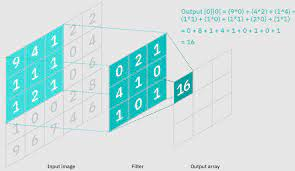
\includegraphics{index.jpeg}
	\caption{Structure Of Convolution Operation (Image Source \cite{convImg})}
    \label{fig:conv}
\end{figure}

In addition to convolution, we have a few other operations that are used in CNNs that account for small portion of computation , the following are supported by the inference engine:

\section{Pooling}

In CNNs, a pooling layer takes a section of the feature map, performs some reduction operation like average, maximum etc. to yield a scalar value. This operation is called pooling. Mathematically, a n$\times$n pooling with a stride of s is given by:

\begin{equation*}
	Output[r,c,chl] = reduce(Operator,Input[(r-1)s+1:(r-1)s+n,(c-1)s+1:(c-1)s+n,chl])
\end{equation*}

where the reduction can happen using any associative operator, like sum, maximum, minimum.

Our engine supports the most common pooling seen, which is maxpooling for n=2 and s=2, which computes the outputs as follows:
\begin{equation*}
	Output[r,c,chl] = reduce(maximum,Input[2r-1:2r,2c-1:2c,chl])
\end{equation*}


\section{Residual and skip connections}

Residual and skip connections are an important component of modern deep learning architectures as they help in forwarding information and hence, context over distant layers without passing the weights through non-linear activations, and were introduced in the ResNet architecture \cite{ReNet}. The former involves an element-wise summation of two tensors to give the resultant tensor. The latter, on the contrary, concatenates the two tensor maps along a fixed axis (generally the channels) to form the output.

\section{Transpose convolution}

Also known as deconvolution, this operation helps in upsampling of the featrure maps. This is done by adding intermediate zeros between the elements of each feature map to give a much larger feature map,on which a regular convolution operation is performed to give the resulting output tensor.

\section{Non-linear activation}

Non-linear activation functions are applied at the end of each compute layer to improve the model's ability to learn from the dataset. Common activation functions include sigmoid, tanh and Rectified linear unit (ReLU).


Mathematically, we have the following:

\begin{equation*}
	tanh(x) = \dfrac{e^x - e^{-x}}{e^x + e^{-x}}
\end{equation*}
\begin{equation*}
	sigmoid(x) = \dfrac{1}{1 + e^{-x}}
\end{equation*}
\begin{equation*}
	ReLU(x) = x*I_{x>0}
\end{equation*}
where, 
	$I_a$ is the indicator variable which takes value 1 if a is true else 0


\section{Our Architecture}

Since the goal of the project is to highlight the efficiency of the engine to accelerate ML tasks, we use a trimmed down version of the UNET architecture \cite{UNET} as we are not concerned with the performance of the model itself. Note that this trimming doesn't affect the hardware's performance or its ability to execute the functionality of the original architecture, but reduces the compute workload for demonstration. The modified architecture is described by the pseudocode provided here:

\begin{comment}
\begin{figure}[h!]
    \centering
    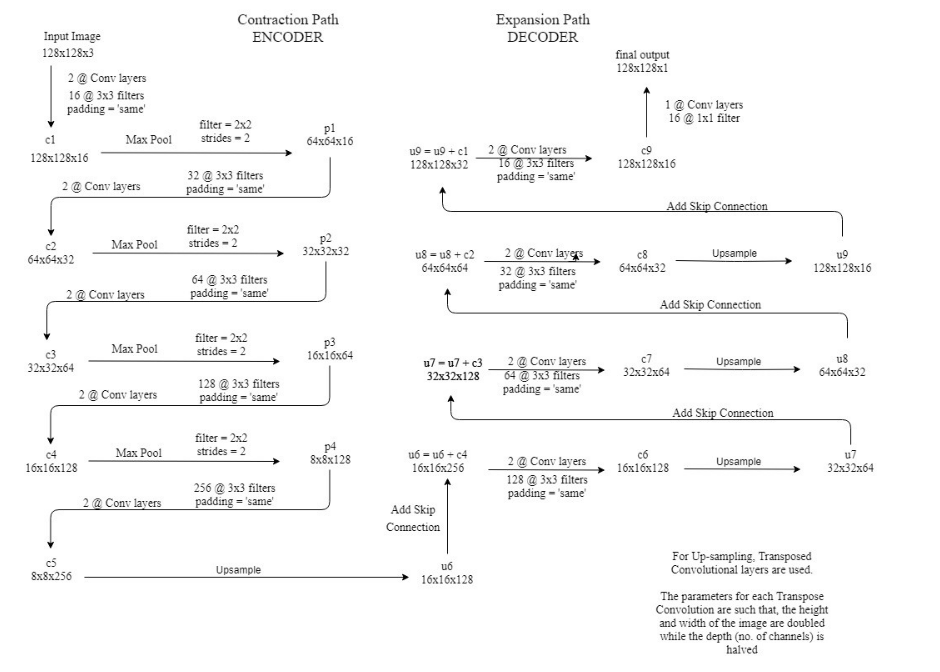
\includegraphics[width=\textwidth]{Screenshot from 2022-10-12 10-38-50.png}
    \caption{Architecture Of UNET Implemented}
    \label{fig:myUNET}
\end{figure}
\end{comment}


\subsection{Pseudocode}\label{pseudocode}

Algorithm~\ref{Algo:UNET} describes the implementation of UNET (the parameters used in each function calls are not shown here).

\begin{algorithm}
	\caption{Pseudocode for UNET implementation}
	\label{Algo:UNET}
	\begin{algorithmic}[1]
    \State $T \gets read\_input\_tensor()$
    \State $K \gets read\_kernels()$
		\For {iter = [1:3]}
        \State convolve(T,K[2*iter-1], T')
        \State relu(T')
        \State convolve(T',K[2*iter],T)
        \State relu(T)
        \State $R[iter] \gets store(T)$
        \State pool(R[iter], T)
    \EndFor
    
    \State convolve(T,K[7],T')
    \State relu(T')
    \State convolve(T',K[8],T)
    \State relu(T)
    
	\For {iter = [1:3]}
        \State convolveTranspose(T,K[6+3*iter],T')
        \State relu(T')
        \State concatenate(T',R[4-iter],T)
        \State convolve(T,K[7+3*iter],T')
        \State relu(T')
        \State convolve(T,K[8+3*iter],T')
        \State relu(T')
    \EndFor

    \State convolve(T',K[18],T)
    \State sigmoid(T)
    \State send\_output\_tensor(T)

	\end{algorithmic}
\end{algorithm}

\begin{comment}
\begin{Verbatim}[numbers=left,commandchars=\\\{\}]
\label{Algo:UNET}def UNET:
    T = read_input_tensor()
    K = read_kernels()
    for iter in [1:3] do
        convolve(T,K[2*iter-1], T')
        relu(T')
        convolve(T',K[2*iter],T)
        relu(T)
        R[iter] = store(T)
        pool(R[iter], T)
    endfor
    
    convolve(T,K[7],T')
    relu(T')
    convolve(T',K[8],T)
    relu(T)
    
    for iter in [1:3] do
        convolveTranspose(T,K[6+3*iter],T')
        relu(T')
        concatenate(T',R[4-iter],T)
        convolve(T,K[7+3*iter],T')
        relu(T')
        convolve(T,K[8+3*iter],T')
        relu(T')
    endfor

    convolve(T',K[18],T)
    sigmoid(T)
    send_output_tensor(T)
\end{Verbatim}
\end{comment}
\subsection{Datatypes Used}

Studies have found that fixed point computation for CNNs can achieve similar accuracies with significantly lower logic utilisation, and thereby boasts of higher resource efficiency \cite{FPGA2,FPGA3}. Hence, we design the engine for a 8-bit fixed point format for storing all the data. The multiplication gives a 16-bit output, which is then accumulated in 32-bit buffers, which is similar to the implementation done in Google TPU \cite{TPU}. The scaling at the end is done using a 32-bit multiplier, from which the appropriate 8 bits are selected for write-back into the next stage.  Use of fixed-point data simplifies the hardware, allowing faster inference. The position of the decimal and scale valies are software controlled, and appropriate scaling and shifting can be done after each stage to ensure that the format is maintained with minimum loss of accuracy.


\chapter{Design}\label{ch:3}

In order to perform inference tasks successfully, the engine must have the ability to perform operations like concatenation, convolution, zero-padding, max-pooling, non-linear activation (relu) and transpose convolution. We show the block diagram indicating the modules used and the flow of data within the system through Figure~\ref{fig:block_dia}. On the left are the set of input modules and the kernel modules. They are responsible for fetching the inputs and the kernels from the memory. They are supported by the readModules which are connected through a deadlock prevention mechanism. The fetched data is forwarded through pipes to the convolveCore, where the bulk of the computation occurs. The partial sums are then accumulated in the accumulator, after which the outputs are generated through scaling and applying activation functions before being written back to the memory using the sendModules. The design and working of individual modules are described in the following sections.


The primary requirement of the engine is that it should be able to perform all operations listed above with a high throughput. In order to do so, a core unit that can perform multiple parallel MACs is important. Since the core operation of CNNs is convolution, and all other operations are generally done before or after convolution, we cascade the layers to generate hardware that executes other operations as a preprocessing or postprocessing step to the execution of convolution layer. By doing so, we eliminate the need for a memory access after every layer, and hence, the latency of operations improves significantly. We call the combined execution of the preprocesssing, one layer of convolution and postprocessing as a stage. By structuring the engine in this manner, we are able to perform an end-to-end UNET implementation in 18 stages, as opposed to the 38 layers required during training. In addition to the parallelism to generate high throughput, we require minimum data movement across the processing elements to ensure low resource consumption and interconnect delays. So, we use a 384 processing element streaming architecture as described in Section~\ref{sec:convCore}.



\begin{figure}[h!]
    \centering
	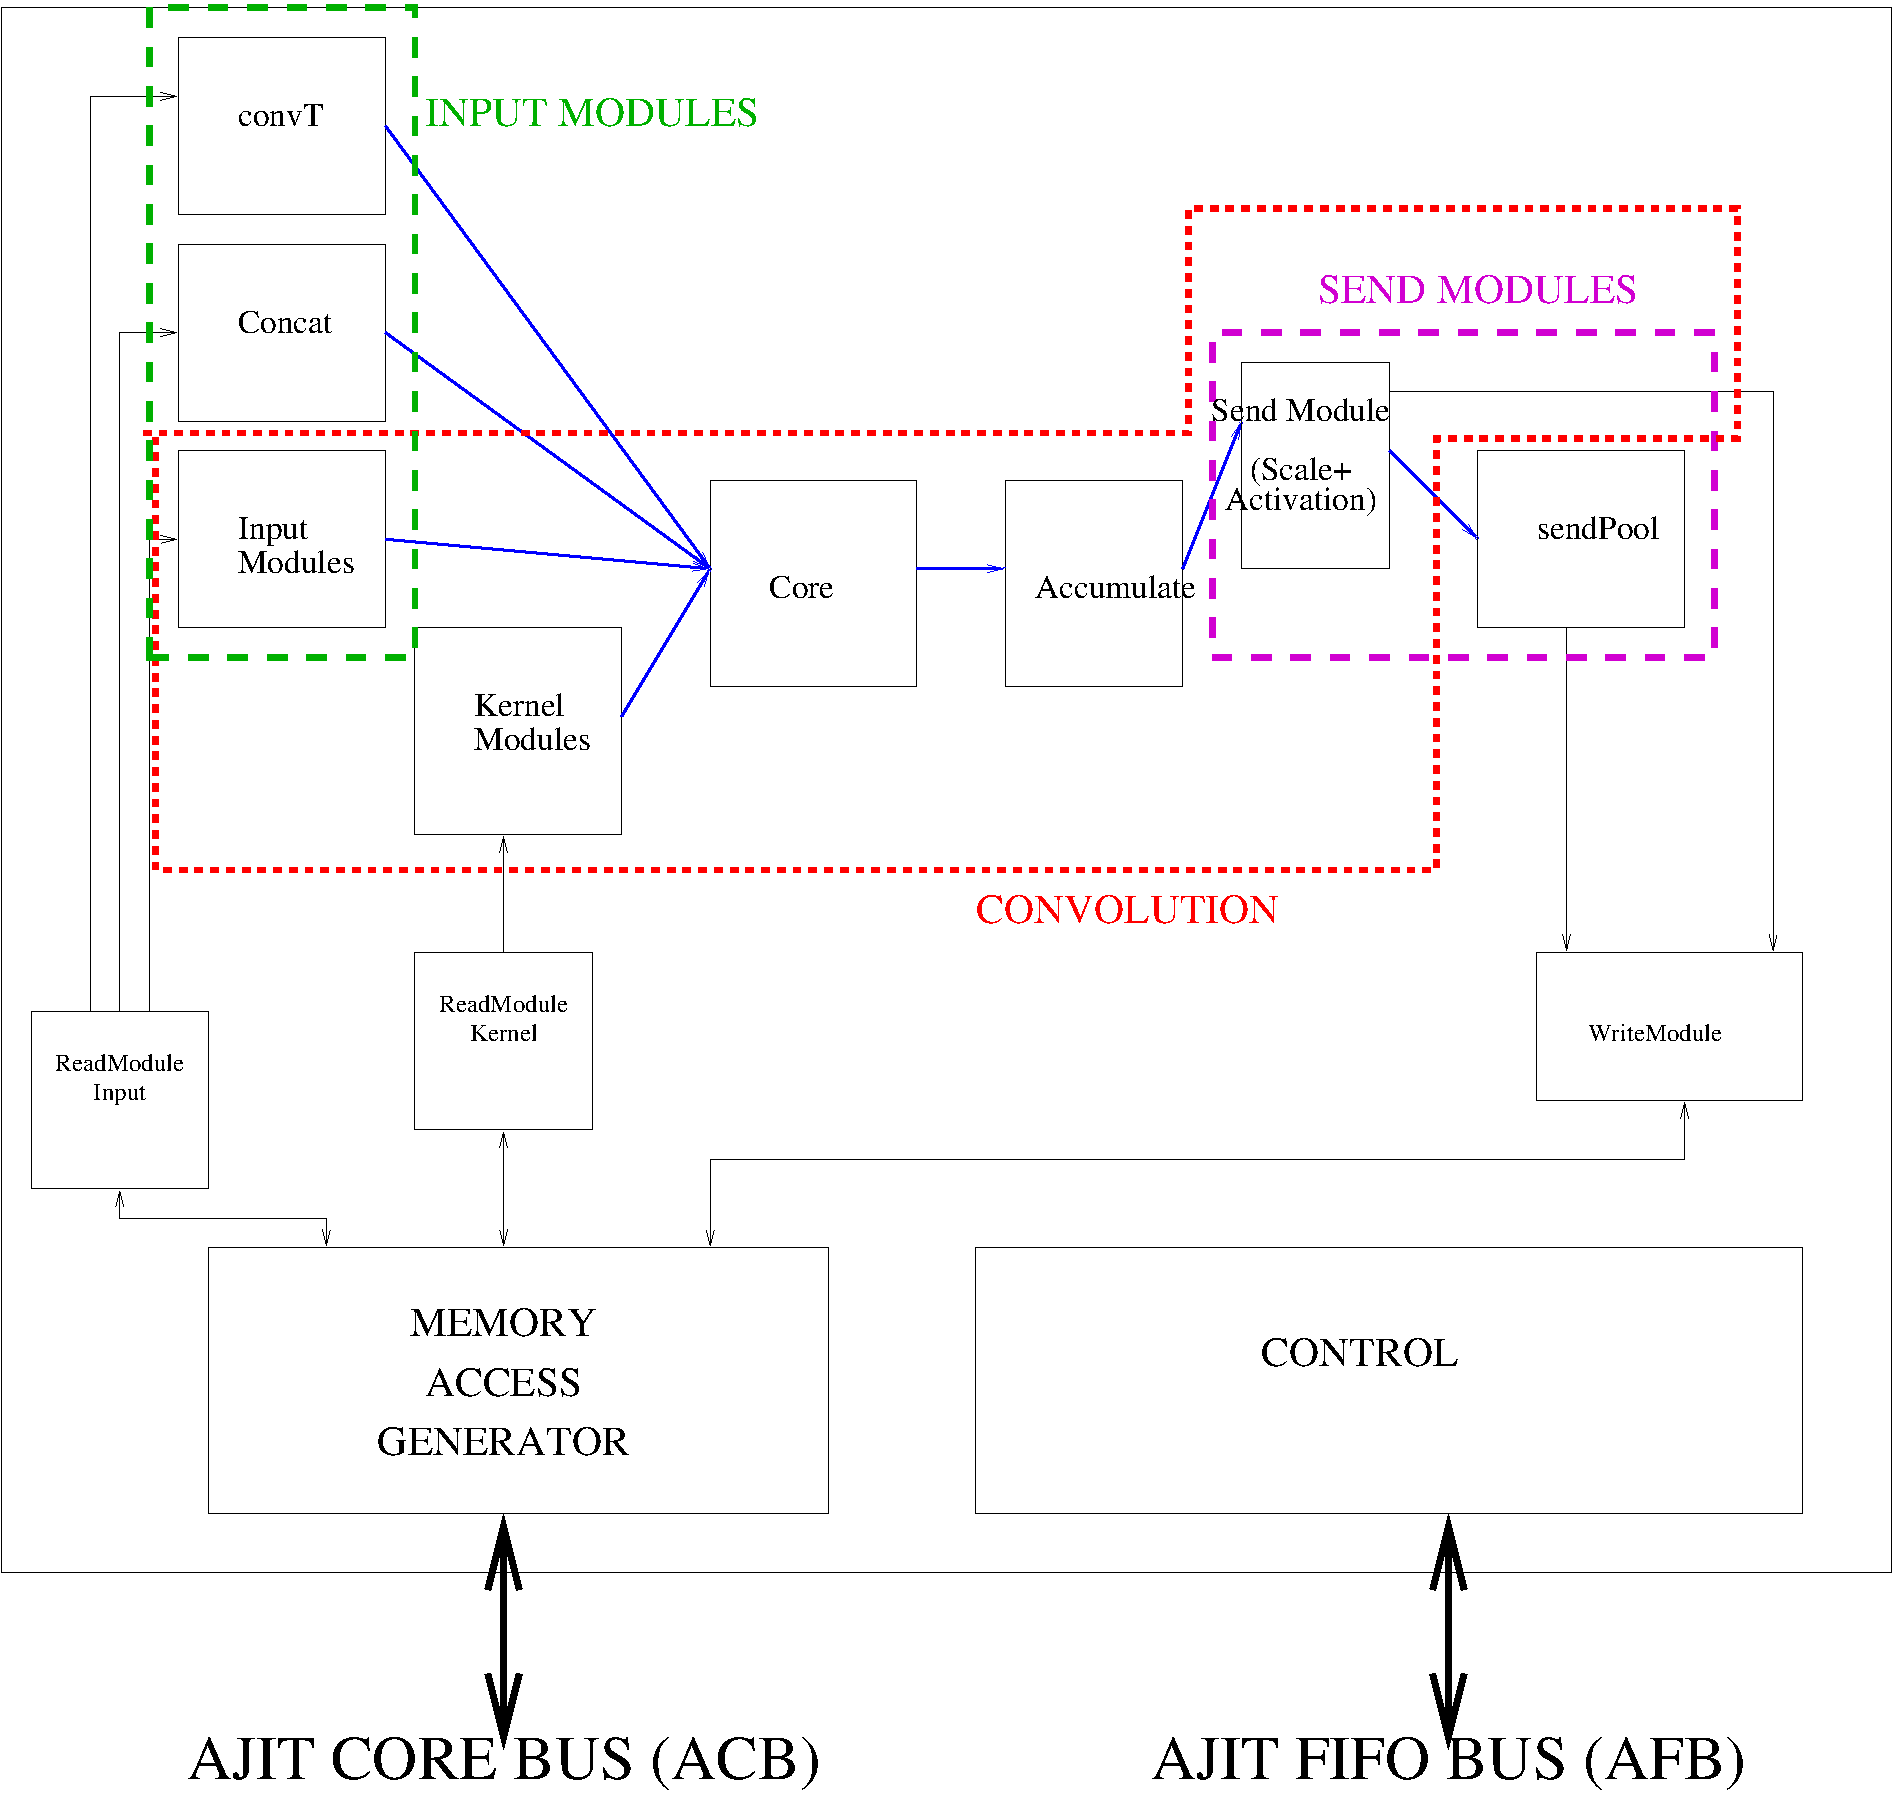
\includegraphics[width=\textwidth]{updated_modules.pdf}
    \caption{Block Diagram For The System Implementation}
    \label{fig:block_dia}
\end{figure}

An important design consideration while developing the inference engine is the memory sub-system. For UNET, we have observed that the tensor sizes can go over 3MB, and the largest kernel exceeds 2MB in size. It is infeasible to have buffers storing all the information for a given stage. However, we can note that for a 3x3 convolution, an output at row $r_i$ and column $c_j$ is affected only by inputs in rows $r_{i}$ to $r_{i+2}$ and columns $c_{j}$ to $c_{j+2}$. Hence, as we increment the output location, we move to the next input element. This allows us to fetch inputs by streaming them through the pipeline to process the outputs.


However, each input is used $r_k*c_k*chl_o$ times throughout the execution, which means that the memory IO requirements for input fetching could go over 200 million accesses for a given stage, with each input being fetched over 4500 times. This could lead to a huge load on the memory bandwidth, and will undoubtedly slow down the system. This calls for the need of a system to reuse the inputs completely before they are discarded. The importance of reuse of data is most noticable for kernel data, which are used as much a s$r_*c_i$, which can be in excess of 50000 for feature maps of size 224*224 seen in UNET implemented by us. For layers having larger image size like 572*572 used in the first stage original architecture \cite{UNET}, each kernel value is used a staggering 327184, making it extremely necessary to optimise on the kernel reuse.


The most direct way is to buffer the kernels directly. This method is feasible if the size of the kernels are small, however real life kernels can be extremely large. An example is the kernel used in the UNET architecture just before the upsampling block. This kernel has $3*3*1024*1024$ elements, which will require a storage space of 9MB using 8-bit data.


To mitigate this issue, the kernels are partitioned into units that can be stored on the on-chip FIFOs. The partitioning is done to accommodate as many output channels as possible in the buffers, thereby minimising the number of partitions. The inputs have to be streamed once for every kernel partition. Since the number of times each input is fetched is equal to the number of partitions, it is imperative to ensure that the number of partitions are kept as low as possible to improve system performance. Currently, 768 KB of kernel buffer is provided, which keeps the maximum number of partitions as 3 for the architecture deployed.


The design involves two aspect - the critical component involving the convolution core, internal buffer management and memory IO, and the non-critical components for auxiliary tasks like concatenation, maxpooling, padding and applying non-linear activations.


\section{Algorithm}

Rewriting Algorithm~\ref{Algo:conv}, we get Algorithm~\ref{algo:convCore}. This is the one that is implemented by the two modules (blue denotes convolveCore specific tasks, red denotes accumulator tasks).

\newcommand{\getsCustom}{$\gets$}


\begin{algorithm}
	\caption{Algorithm for execution of convolution in the engine}
	\label{algo:convCore}
\end{algorithm}
\vspace{-1cm}
\begin{Verbatim}[numbers=left,commandchars=\\\{\}]
\textcolor{brown}{// Two output rows at a time}
for r = 1:2:r_o do
	for c = 1:c_o do
		\textcolor{brown}{// 8 output channels simultaneously}
		for co = 1:8:chl_o do
			\textcolor{red}{partial_sum[2,8] = 0}
			for c' = 1:c_k do
				\textcolor{brown}{// 8 input channels at a time}
				for ci = 1:8:chl_i do

					\textcolor{brown}{// The below part happens in one loop of the core}
					\textcolor{brown}{// Hence we replace for with for_unrolled which signifies}
					\textcolor{brown}{// that the loop is unrolled over the range of its iterators}

					\textcolor{brown}{// Temp variable for 384 multiplications}
					\textcolor{brown}{// which are accumulated and reduced to 16 partial sums}
					\textcolor{blue}{tmp[2,8,8,3] \getsCustom 0}
					\textcolor{blue}{tmp_reduced[2,8] \getsCustom 0}
					\textcolor{blue}{for_unrolled co' = co:co+7 do}
						\textcolor{blue}{for_unrolled r' = 1:r_k do}
							\textcolor{blue}{for_unrolled ci' = ci:ci+7 do}
								\textcolor{blue}{tmp[1,co',ci',r'] \getsCustom input[r+r'-1,c+c'-1,ci']*kernel[co',r',c',ci']}
								\textcolor{blue}{tmp[2,co',ci',r'] \getsCustom input[r+r',c+c'-1,ci']*kernel[co',r',c',ci']}
							\textcolor{blue}{end_unroll}
						\textcolor{blue}{end_unroll}
						\textcolor{blue}{tmp_reducei[1,co'] \getsCustom sum(tmp[1,co',:,:])}
						\textcolor{blue}{tmp_reducei[2,co'] \getsCustom sum(tmp[2,co',:,:])}
					\textcolor{blue}{end_unroll}
					\textcolor{blue}{endfor}
					\textcolor{blue}{sendToAccumulator(tmp_reduce)}
					\textcolor{red}{receiveFromConvolveCore(tmp_reduce)}
					\textcolor{red}{partial_sum \getsCustom partial_sum +  tmp_reduce} \textcolor{brown}{// Element wise sum}
				endfor
			endfor
		endfor
	endfor
endfor
\end{Verbatim}

\section{Critical components}

In our design, we have two critical components which are responsible for executing the computation. These are convolveCore and the accumulator. We describe their organisation and features here.

\subsection{convolveCore}\label{sec:convCore}


The convolveCore is the most critical component in the accelerator. The purpose of the module is to ensure that a large number of computations can be carried out simultaneously to facilitate the acceleration we desire. In order to do so, the core unit is designed as a 2*8*8*3 multiplier system. This provides a theoretical peak of 768 operations per clock cycle. The organisation of the multiplier array was chosen to allow for two rows of ouputs processed 8 channels at a time, with support of kernels upto 3 rows, and inputs received 8 channels at a time. The use of 8 input/output channels was motivated by the use of 8-bit datatype, allowing us to process and write-back double-words at a time and improving memory performance. Also, two rows of outputs are delivered simultaneously, facilitating easier maxpooling.


The processing elements can be viewed as 6 logical sections of 8*8 multipliers arranged as shown in Figure~\ref{fig:core}, and represents the unrolling seen on lines 20,22 and 23 of Algorithm~\ref{algo:convCore}. The inputs and kernels are multiplexed such that the first three sections compute the partial products for the first output row, while the next three sections produce the partial products for the second output row. Since convolution uses a sliding kernel window, the kernel remains the same across each row, while the input is shifted by a single row. This implies that the second and third inputs are utilised by two sections each.


Each logical section can be broken down into an 8*8 processing element grid, where there are 8 sections corresponding to the 8 output rows. All of them receive separate kernel values but the same inputs. Each sebsequent block receives 64-bit values, which are sliced into 8 8-bit values and a dot product over them is computed. This corresponds to the for\_unrolled loop in the algorithm described in line 21 of Algorithm~\ref{algo:convCore}. The outer 8 sections each represent a unit from the unrolling of line 19 of the same algorithm.


\subsubsection{Data Buffering And Reuse}

During the processing of one stage, the core module iterates over the above computation multiple times as mentioned in lines 2,3,5,6 and 8 of Algorithm~\ref{algo:convCore}. This amounts to a total of $\dfrac{r_o*c_o*chl_o*chl_i*c_k}{128}$ iterations. Furthermore, in order to release the partial sum from the storage buffers immediately, each output must be computed before the next one is started, which leads to lines 6 and 8 being executed before the outer loops. Thus, the flow of inputs through the core module involves passing all the channels corresponding to the given row and column before moving to the next column. After a column c is used for computaion, the next $c_k-1$ columns are sent, after which again c+1 to $c+c_k-1$ are sent, and so on. For $c_k$ =  3, all columns are used 3 times before the next row is sent in. Since the outputs are processed 2 rows at a time, the input is sent at intervals of two rows, i.e. the first input pipe (core\_ip1) will receive input rows 1,3,5, and so on, while the second input pipe (core\_ip2) will receive input rows 2,4,6 etc . 


Looking at the flow of kernels, they have to be sent corresponding to the inputs they multiply with, and so, they are sent channel by chaanel, followed by columns. Since all rows of the kernel are sent simultaneously (they are at most 3), the kernels iterate over the output channels, for each of which the same input needs to be streamed again.


Thus, we observe that each input is being used $c_k$ times for different output columns, $r_k$ times for different output rows, and $chl_o$ times for different output channels, and the kernel is reused $c_o*r_o$ times as it slides or each output element of a feature map. Out of which, the architecture reuses the input 1.5 times and kernel twice. If there are no mechanisms for the inputs and kernels, we will require a very high memory bandwidth of $\dfrac{48}{1.5}$ accesses per clock for inputs, and $\dfrac{48}{2}$ accesses for inptus for kernels, leading to 56 memory accesses every clock cycle) to maintain full rate of execution.


As the memory bandwidth is limited to 1 access per clock cycle, we provide the core with pipes that serve as buffers for reuse of data. There are 4 pipes of depth 256 (total of 8KB buffer) for buffering inputs, and are designed to store 3 columns of input data. This improves the input reuse by a factor of $3*chl_o$ by reusing the inputs across all output channels and kernel columns, bringing the average input bandwidth requirement down significantly to around $\dfrac{48}{4.5*chl_o}$, which in the range of 0.02 - 0.2 accesses every clock cycle as $chl_o$ ranges between 64 and 512.


Observing that the kernel is reused a few thousand times, it makes sense to store the kernels completely on chip as the added storage is justified by the immense savings in memory accesses. To facilitate that, 24 pipes of depth 4096 (32KB each for a total of 768KB) are used to provide 3 rows of kernels and 8 output channels at a time. Thus, we ensure full reuse of kernels and bring down the average kernel bandwidth requirement drastically. In some cases, the kernel size may exceed the buffer sizes. In such scenarios, the output is partitioned based on the number of channels, and a few channels are computed at a given point in time. Thus, only the kernels corresponding to the output channels are buffered. The partitioning is done in a way to ensure maximum use of the kernel pipes, which will lead to the minimization of the number of times the input is fetched, since all the inputs are fetched as many times as the number of kernel partitions.


\begin{figure}[h!]
    \centering
    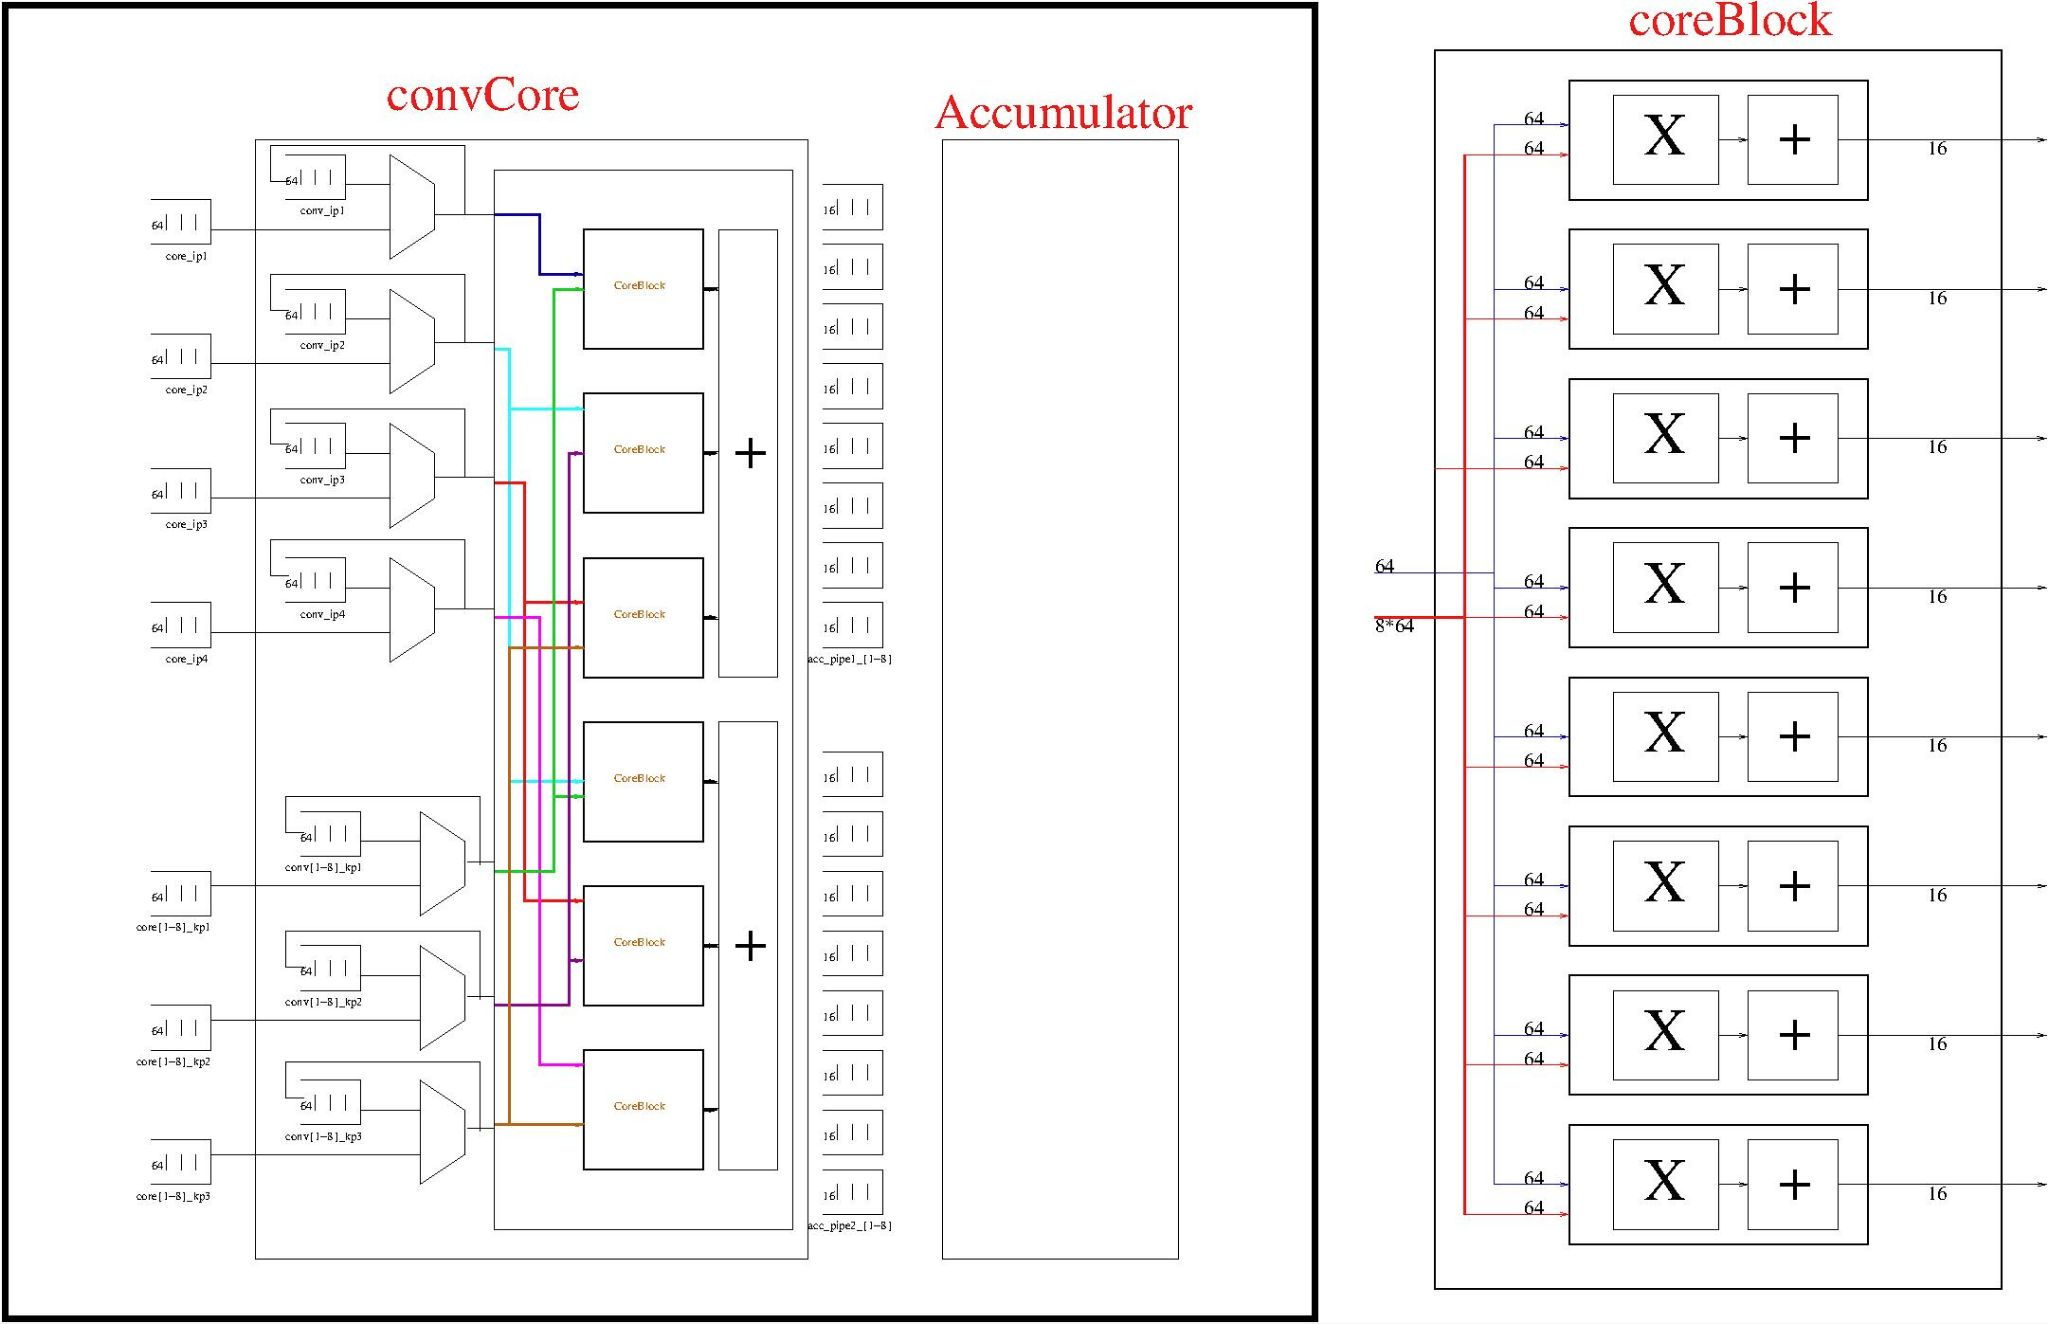
\includegraphics[width=\textwidth]{Core.jpg}
    \caption{Organisation of the critical modules - convolveCore and accumulator}
    \label{fig:core}
\end{figure}

\subsection{Accumulator}

The accumulator is implemented independent of the core unit. This is done to improve the performance of the system as each iteration of the core can run in one clock cycle. The accumulator reads the values and accumulates until count equals the parameter acc\_count, which corresponds to the number of product of the number of channels and columns of the input required to get a output. After that, the counter and the accumulated value resets and waits for the next set of partial sums to produce the next output. The accumulator unit is capable of handling 16 sets of partial sums every clock cycle.


The accumulator reads 16 output values across 2 rows and 8 output channels, and maintains partial sums that are 32b wide, which is the same used in TPUs \cite{TPU}. On completion of every accumulation, the data is forwarded to the sendModule/sendModule8/sendPool through sendPipes for further processing and writeback to the memory.


\section{Non-critical components}

Convolution module is a collection of multiple smaller modules, and has the ability to perform zero-padding, maxpool, concatenation, transpose convolution and non-linear activation in addition to its core functionality. This can be done as all the above operations are linear in their mapping from input to output, and hence any stream can be modified insitu to get the modified stream. This facilitates the use of specialised input/output modules to achieve the above operations.


Thus, the overall scheme reduces to the design of an all-purpose core which can be integrated with each of the input/output configurations to get the desired functionality. The convolution module can perform 8-bit multiplication on int8 data, with 32 bit accumulation. The accumulator is kept as a separate entity than the multiplier core to facilitate full-rate execution as this leads to no data dependency in the multiplication unit.


\subsection{Input Modules}

In order to reduce the number of memory accesses and provide a steady stream of data to the convolution core, a series of modules were implemented to deliver the inputs at the best possible rate based on the operation to be performed.


This module reads the input tensor from the memory, and sends it to the core for processing. The modules are designed to fetch two input rows at a time. This is done due to two reasons:
\begin{enumerate}
\item Keeping the number of rows to two allows us to fetch the input data only once per kernel partition in a layer instead of two times required by the convolveCore, leading to full reuse. As we increment the number of rows by two, we forward the same data twice to the convolveCore using the singleFetch module described below.
\item Since the output produces two rows at a time, having two input rows provides an opportunity to cascade multiple engines to eliminate intermediate memory accesses.
\end{enumerate}

All the input modules have support for padding with zeros by sending in zeros at the desired positions. This enables us to prevent restructuring of the tensor to enable zero-padding. They call a two concurrent submodules to fetch one row each - the first module handles the odd numbered rows, while the second handles the even numbered rows. The modules ensure that the zeros created due to padding are transmitted to the singleFetch module. We represent the organisation of the input modules in the system in Figure~\ref{fig:inputModules}.


\begin{figure}[h!]
    \centering
    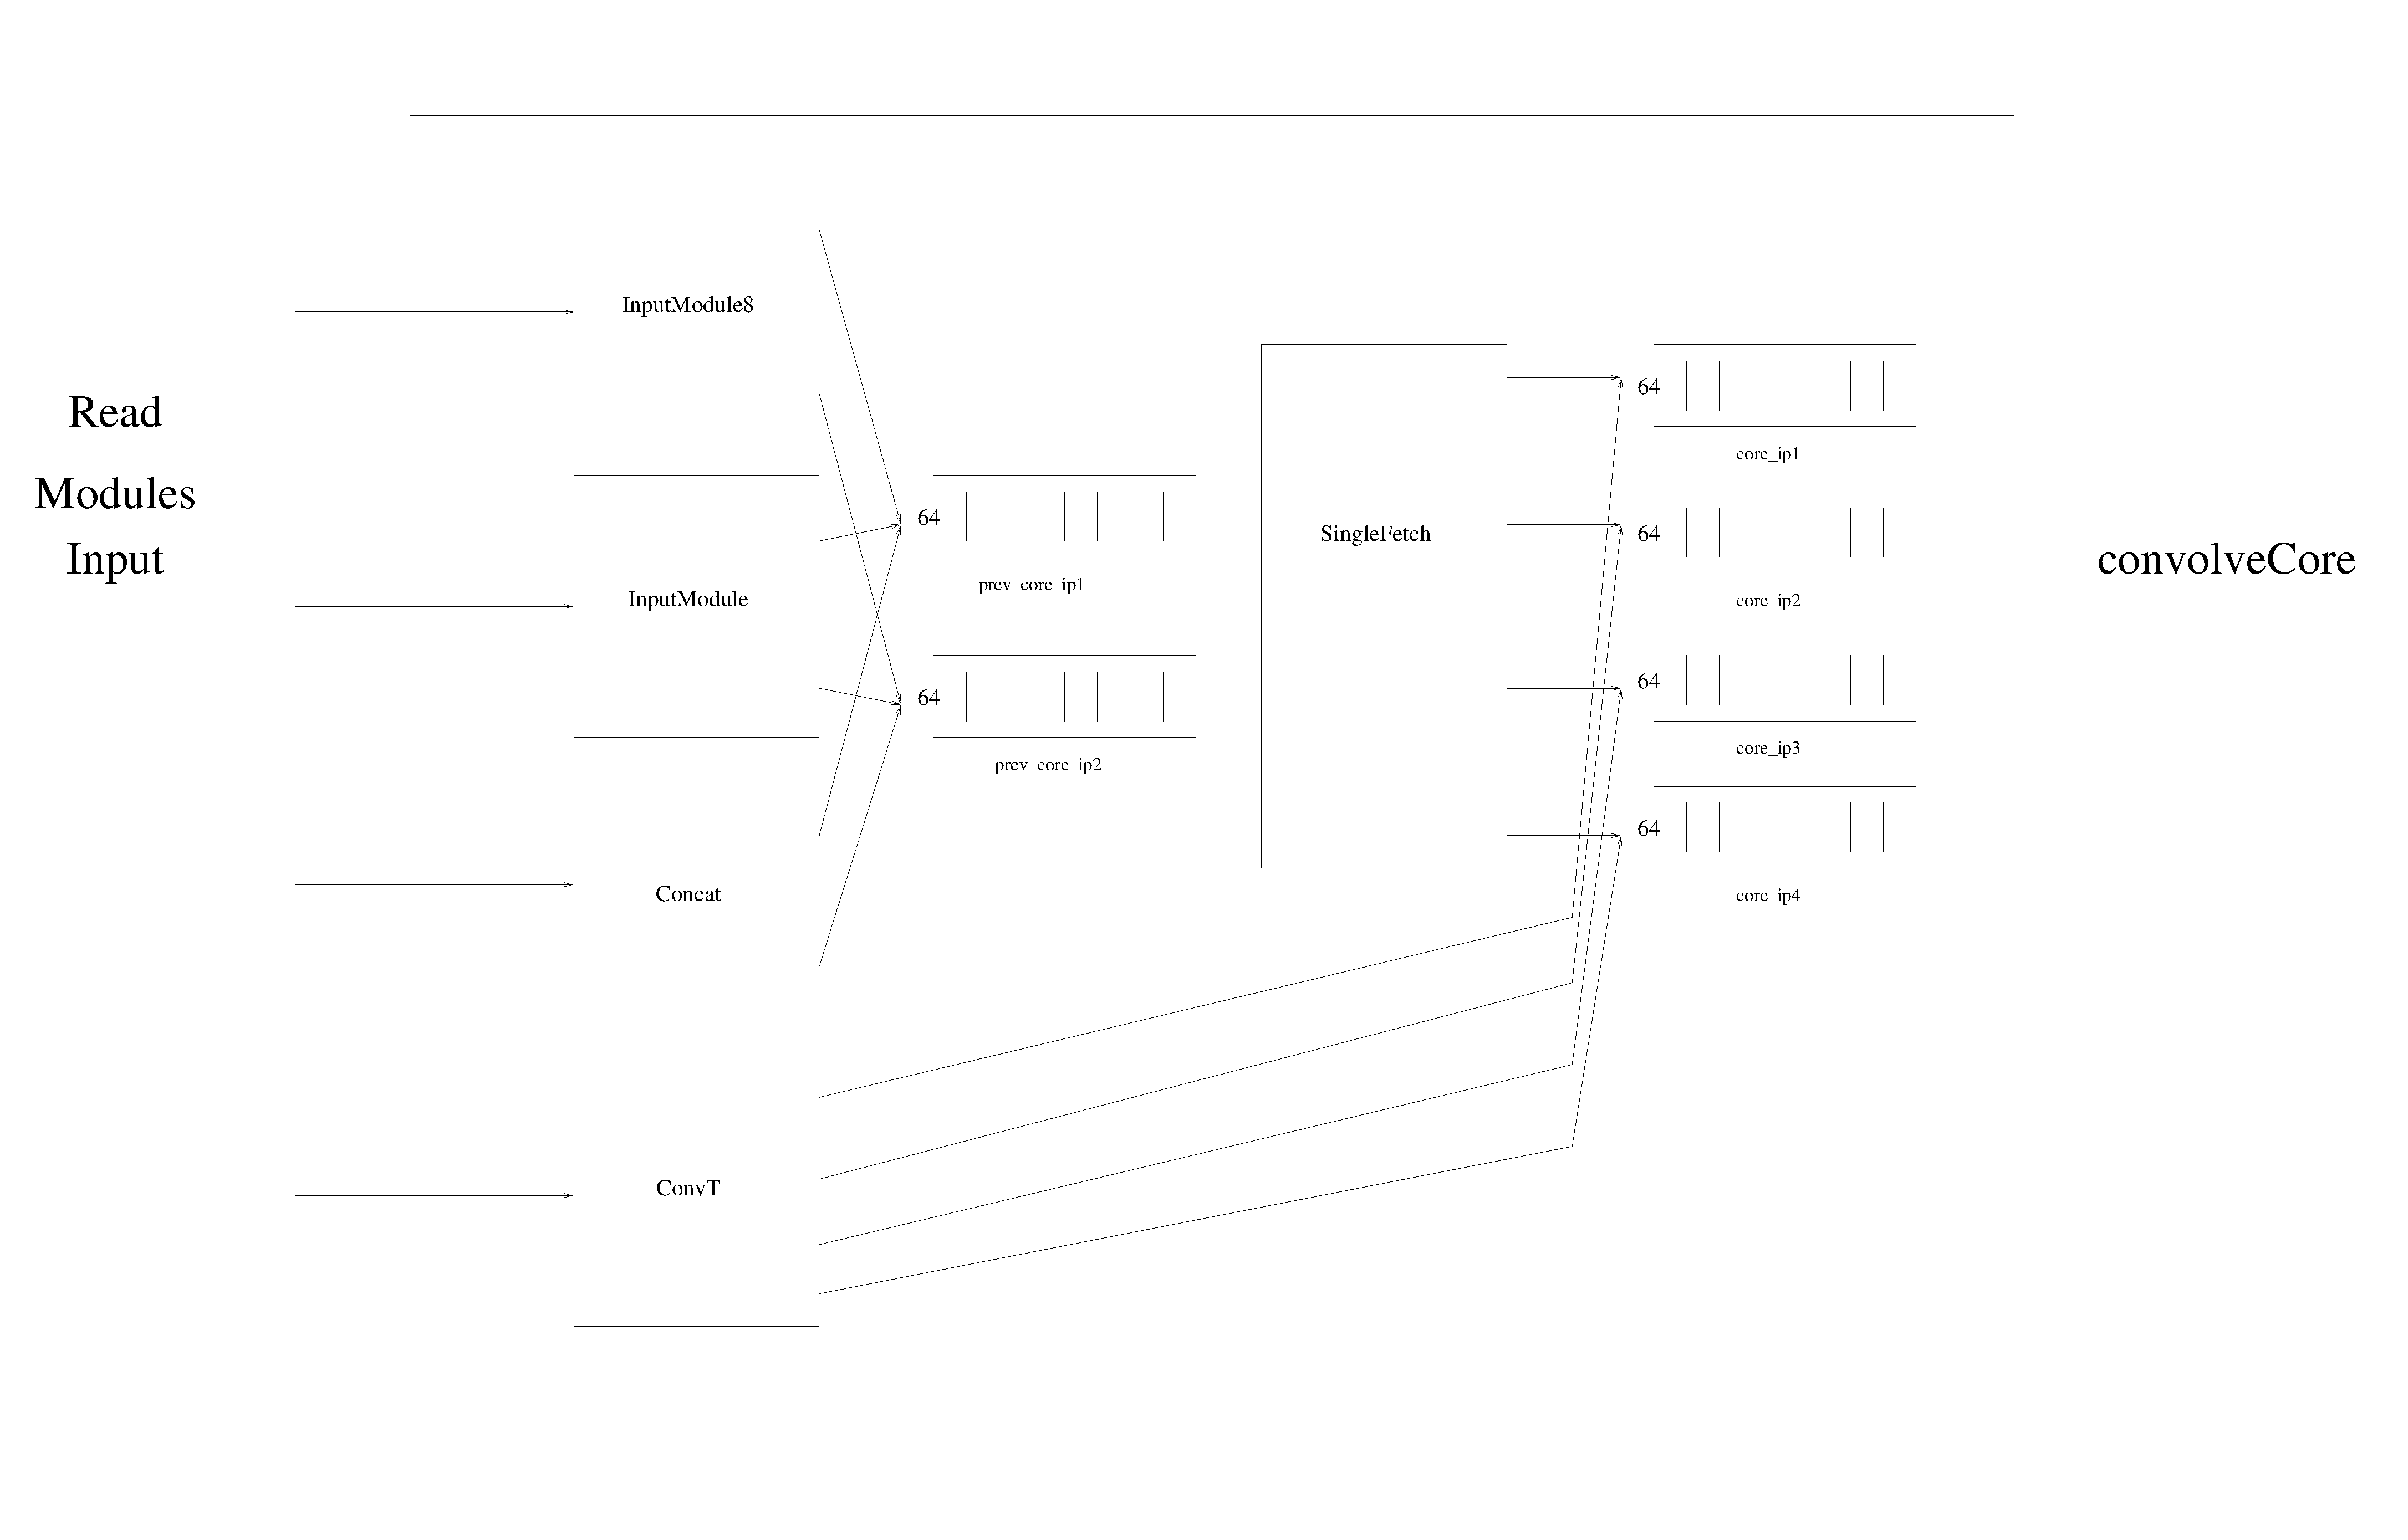
\includegraphics[width=\textwidth]{inputModule.pdf}
    \caption{Organisation of the input modules}
    \label{fig:inputModules}
\end{figure}

\subsubsection{Single Fetch}

As discussed in the convolveCore section, each input has to be streamed twice for correct operation. However, using the singleFetch module, we provide the illusion of the streaming the inputs twice but with a single read for each input. This module reads the first two input rows and buffers them in the FIFOs for the core. At this point, the core blocks due to unavailability of data in the third and fourth input FIFOs. The module sends the next row into the FIFO 1 and 3, and the subsequent one to FIFOs 2 and 4. This way, after an initial delay, it gives the core an illusion that all four rows are available simultaneously, while in reality the last two FIFOs lag the first two by $c_i*chl_i$ elements, which is then corrected when the last row is forwarded only to the third and fourth FIFOs, thereby balancing all inputs.


This way, the number of times each input is fetched is kept to a bare minimum of 1, allowing the core to function at full rate. However, this does require an additional storage to buffer two rows of inputs, which can go upto $2*224*64$ Bytes = 28KB. Since inputs can be much larger, a total of 64KB is provided for row buffering to execute other architectures.

\subsubsection{Unpacking}

One of the other functionalities of the input modules is to unpack of the input, such that each element is channel-aligned, i.e. the first channel is always at the start of the word. This ensures correct operation when the number of input channels is not a multiple of 8. These are useful at the input and output stages of the CNN where the tensors correspond to real-world images and hence have 3 channels.

\subsubsection{Transpose Convolution}

This module is designed to replace convTranspose operation. Transpose convolution involves the following operations:
\begin{enumerate}
    \item Writing the tensor with zeros at an appropriate spacing
    \item Depadding the extra layers in the tensor
    \item Performing convolution operation on the resultant tensor
\end{enumerate}

This input module does the first two steps, which reduces the operands to a form that can be processed by the convCore module. To optimize the performance, the two steps are done simultaneously by not padding with zeros at locations which will get depadded. The padding and depadding happens by addition of zeros at the appropriate rows and between adjacent columns. The module reads in the data from memory, but interleaves it with words having all bits zero to get the desired dilated tensor, which is then forwarded to the compute engine for processing. This module also assumes that the number of input channels is a multiple of 8, and hence, the fetched word is forwarded as it is without unpacking.

\subsubsection{Concatenation}

The input modules can also help in concatenation along the channels to implement skip connections, which are executed by alternately reading columns from the two tensors and sending the data stream to the core. This is done by using two counters for the channels to determine when to switch from one tensor to the next. This interleaving results in the concatenation of the two tensors.


Since concatenation occurs only during the decoding loop, it has inputs and outputs which have channels that are multiples of 8. This permits the module to read whole words from memory at a given point in time and send it as it is as the output. Hence, the module is optimised to forward whole words from one memory address to another.


\subsection{Kernel Modules}

This set of modules is responsible for fetching the kernel data from the memory, and sending it to the core. Like the input module, it can unpack the data channel-wise to ensure channel-alignment, ensuring correct operation when the number of input channels is not a multiple of 8. The kernel data is sent through three pipes, one for each row.


The kernel module makes calls to submodules to fetch kernels for different rows. Since $r_k$ is at most three, the submodules need not fetch alternate rows. The fetch is done channel by channel, and is sent to pipes core$<i>$\_kp$<j>$, where $<i>$ is the core number (corresponds to chl\%8), and $<j>$ is the row number, i.e. different for each submodule.

\subsubsection{Minimum latency and buffer requirements}

The kernel module sends the data to the core using 24 pipes, 3 each for 8 output channels processed together. Since the convolution core requires all 8 cores to have valid kernels, there must be enough space in each pipe to store the data corresponding to one input channel, and hence the \verb|INTERMEDIATE_PIPE_DEPTH| is set to 512, which is more than enough for all requirements. This leads to a total buffer requirement of 96 KB for storing intermediate kernels, and since the input pipes are also parameterised by the same depth, they are supported by a buffer of size 16 KB.


As this module transmits kernel values for 8 channels in parallel, we get loop unrolling with 8 loops unrolled. This also allows the convolution module to start processing quickly as it has the kernels required for first computation ready in minimal time. This reduces the startup latency significantly.

\subsection{Output Modules}

The output modules receives the data from the accumulator, and writes them back into the memory after applying the required operations. If the number of output channels is not a multiple of 8, it packs the data into words before writing it into memory. All the send modules are equipped to perform non-linear activation on the output data which is received from the accumulator through two sets of eight FIFOs each 32bit wide. The organisation of the modules in the system is shown in Figure~\ref{fig:outputModules}.

\begin{figure}[h!]
    \centering
    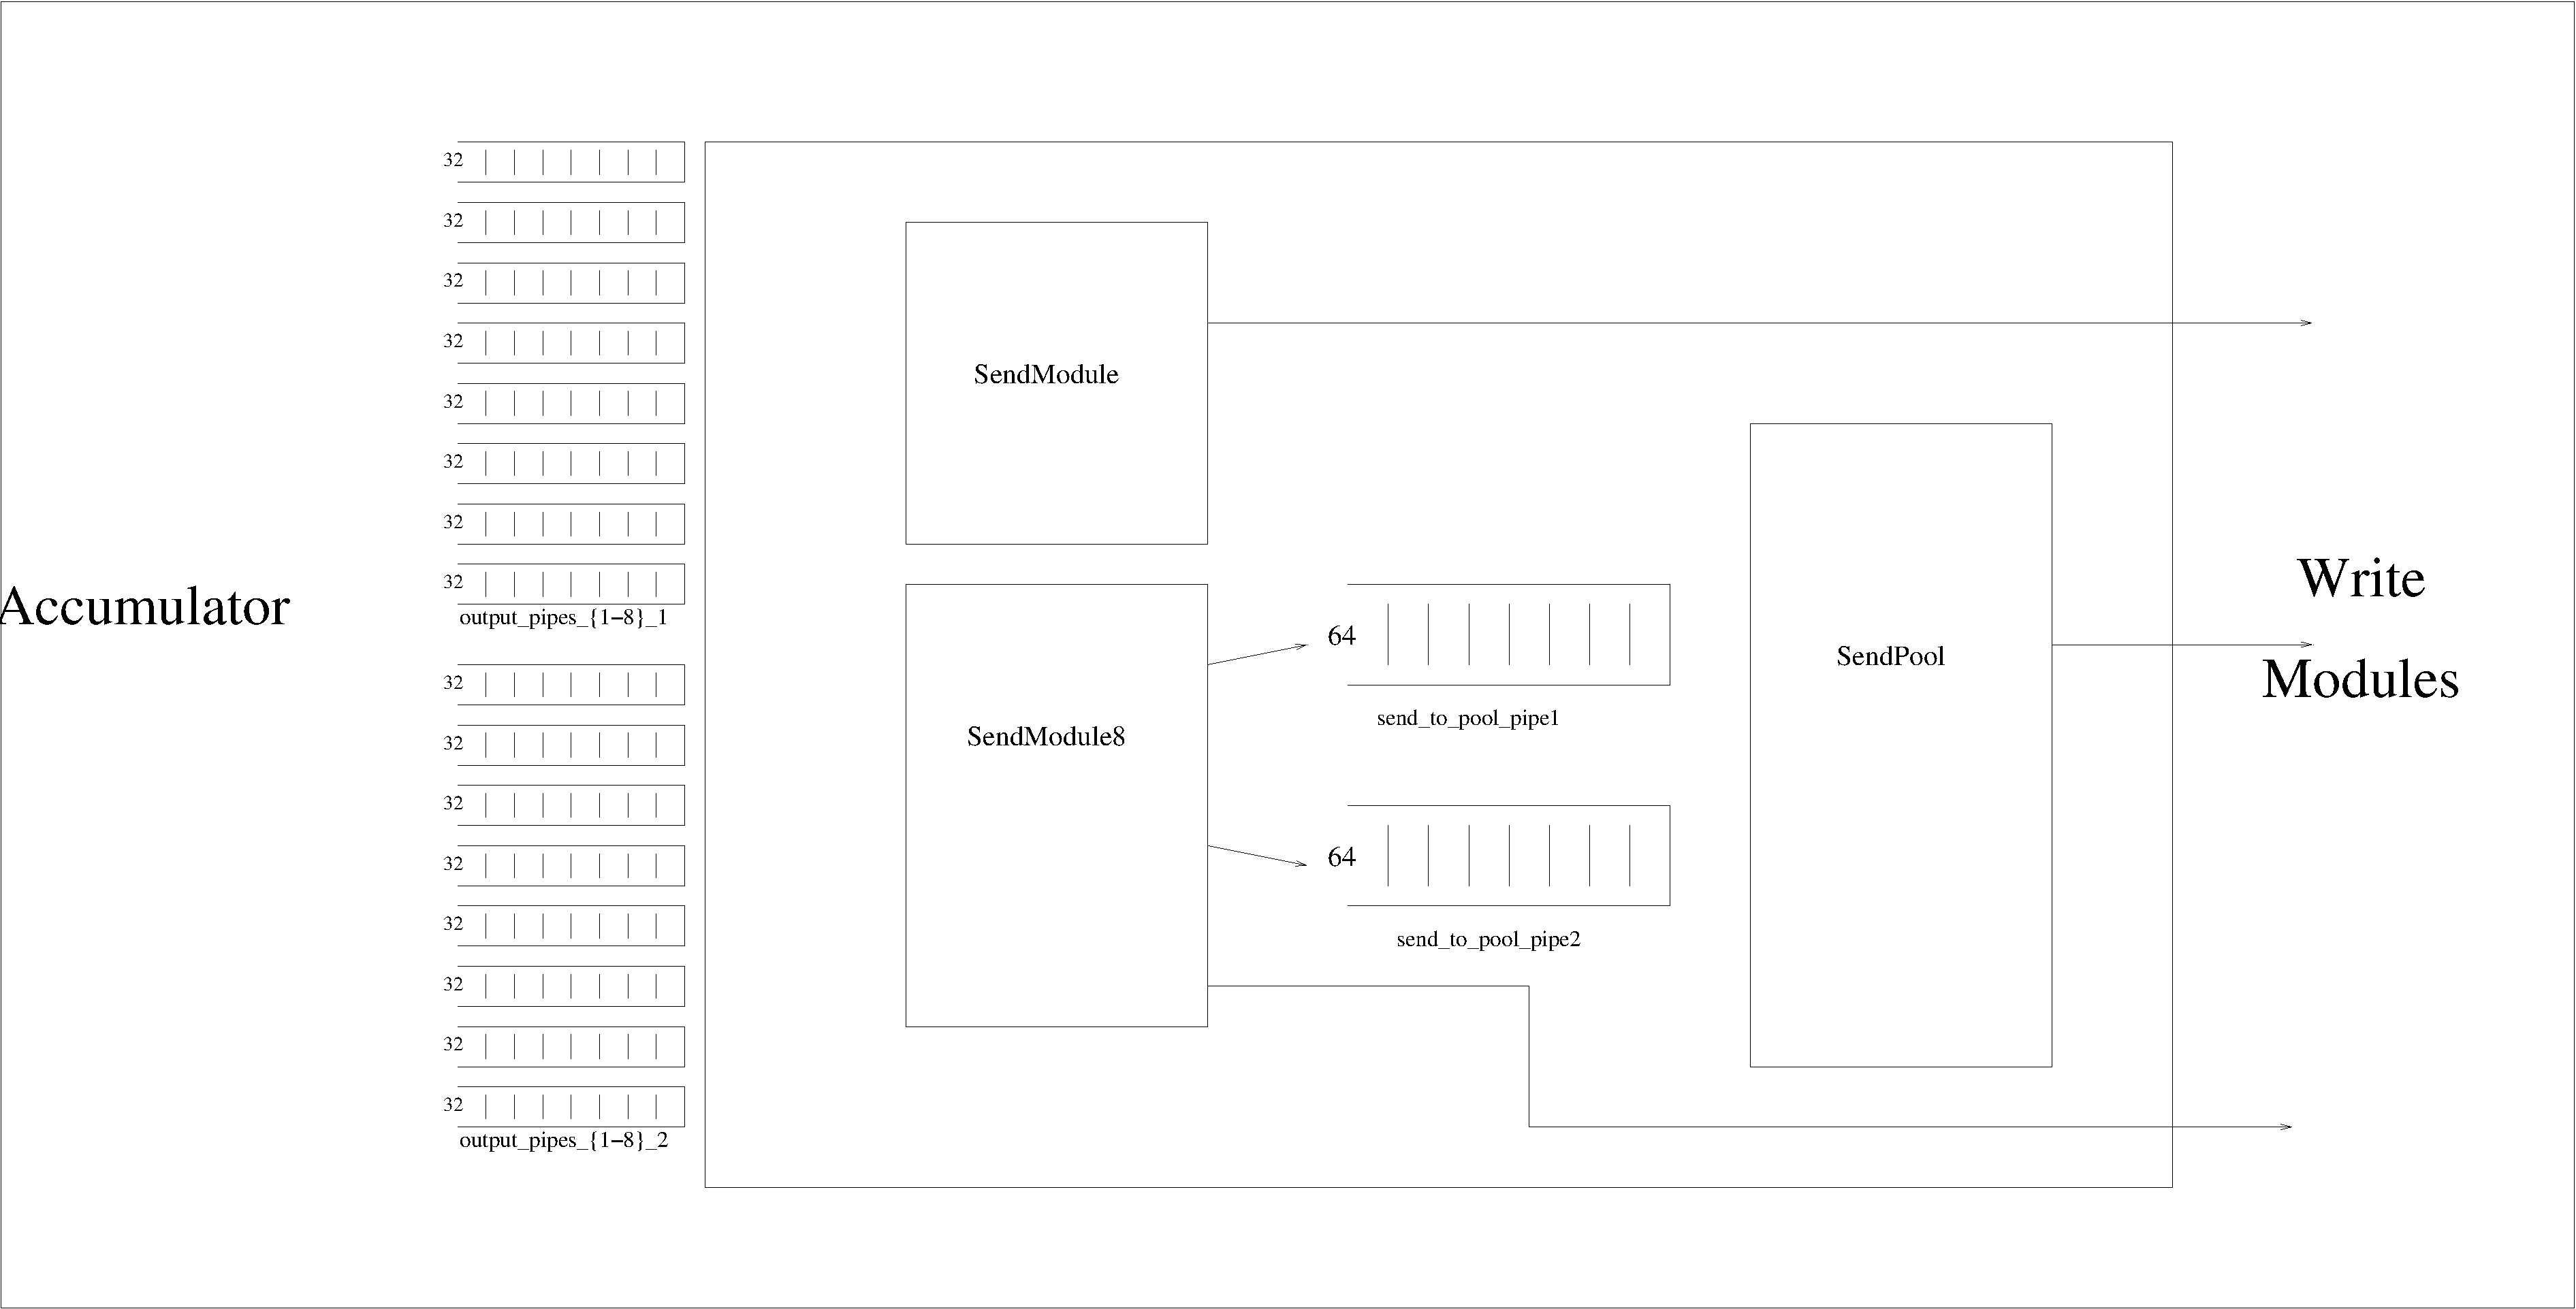
\includegraphics[width=\textwidth]{outputModule.pdf}
    \caption{Organisation of the output modules}
    \label{fig:outputModules}
\end{figure}
\subsubsection{Scaling}

The received data is sent to the scaler module, which translates the data by multiplying it with a 32-bit scale value fixed for a given stage. When the multiplication is done, the data is sent back to the calling module for shifting the data to obtain the final value. This way, high accuracy can be obtained by minimising the loss of information. During a read from the accumulator, 16 outputs are fetched, but only one scaler is used as the accumulator provides data once every $\dfrac{3n}{8}+ 1$ cycles, where n is the number of input channels. Thus, if the number of input channels is 128, writeback happens once every 49 cycles; hence the multiplier associated with the scaler module can be shared across all outputs.

\subsubsection{Non-linear activations}

The module receives the data and performs ReLU if the non-linearity flag for ReLU is set. The operation is performed on the accumulated outputs before the scaling is done. The data is then scaled and truncated before being packed into blocks of 8 elements, which are then written back to the memory. The processing is done two rows at a time. 

\subsubsection{Maxpooling}
The output modules also perform maxpooling after convolution. The pooling operation is done by two modules, the first of which receives the data and performs scaling and shifting. This completes the convolution part and, the intermediate result can be stored if needed. The second module receives the scaled data of two rows and two columns and forwards the maximum of the four values for writeback. Also, since the data is received channel by channel, a small storage of size $chl_o <$ 512B is needed to buffer the partial comparison products. We provide a 2KB buffer for the same.


\section{Auxiliary components}
In addition to the the above modules, we have some auxiliary components that help in the execution of the system.

\subsection{Read and Write Modules}

These modules are an interface between the functional pipelines and the memoryModule, and operate by providing address and/or data along with the appropriate bitmask to the memoryModule for read/write to memory, and delivering the read data back to the calling module in case of a load from memory.


Although There are no cyclic dependencies amongst the core modules, they have one shared resource - the memory which is accessible via the memoryModule. This creates a potential for deadlock as the input module may be blocked by the pipes to the core. This in turn blocks the readModule and hence, the return of data from memory, therefore blocking the memory, which will prevent writeback from the send modules. This will eventually choke the accumulator and the core as the data is still pumped into the send modules but not cleared. In the end, all modules block resulting in a deadlock. Any deadlocks arising due to the blocking of shared resource is mitigated in the read modules using the mechanism shown in Figure~\ref{fig:deadlock}.


The mechanism in the figure work on the fact that the number of live iterations of readModule1 is bound by the pipeline depth 7, and hence, there can be at most 7 entries in the PIPE, and hence, it will never block. Thus, every call to the memory by the readModule1 is eventually returned, thereby preventing any resource contention leading to deadlocks.


It may be noted that there is no need to have a deadlock mechanism for writeModules, since any call to the writeModule eventually returns as the output of the writeModule is not forwarded to a pipe and hence, is never blocked.

\begin{figure}[h!]
    \centering
    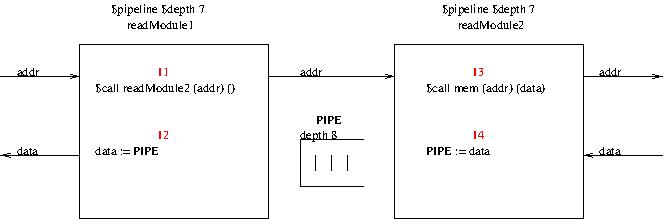
\includegraphics[width=\textwidth]{Deadlock.jpg}
    \caption{Implementation Of Deadlock Free Read Module}
    \label{fig:deadlock}
\end{figure}

\subsection{Memory Module}

The module forms the interface between the engine and the external memory. It receives read/write requests from other modules through their respective read/write modules. It then transmits the 110-bit request to the ahir core bus (ACB), which relays it to the memory controller for memory access. The memory controller sends back a 65-bit response, which includes a 1-bit error flag and 64-bit data, which is forwarded back to the calling module. The memory module provides abstracts the system design from the memory interface. Using an ACB interface, the internal working of the engine just needs to provide the read/write flag, data, address and the bytemask, and wait for the response without having to worry about the actual memory (like BRAM/DRAM) used.

\subsection{Interface To Access The Engine}

Two ever-running daemons control the engine. The first amongst them is the accelerator\_control\_daemon, which resets the registers and starts the worker daemon for operation. It also receives the configuration information from the processor/calling module through the AFB interface, using which it programs the registers.


The second daemon is the accelerator\_worker\_daemon, which polls on the control register R0 until the bits 0 and 2 are set by the calling module. When the condition is met, it reads the other registers and makes a call to the convolution engine via the command:


\begin{Verbatim}
$call convolutionAll (
		ro co ri ci cho chi rk ck
		in1_base_addr in2_base_addr kernel_base_addr out_base_addr1 out_base_addr2
		scale_val shift_val pad pool concat act
		) ()
\end{Verbatim}
where,

\begin{itemize}
	\item ro, co, ri, ci, cho, chi, rk and ck are 16-bit values providing the dimensions of all the tensors and kernels (notation same as in Chapter~\ref{Chap:2})
	\item in1\_base\_addr, in2\_base\_addr, kernel\_base\_addr, out\_base\_addr1, out\_base\_addr2 are the base address for the location of upto two input and output tensors, and one kernel. During pooling, out\_base\_addr2 is used to configure the address to which the pooled outputs are sent. Two input base addresses are used during concatenation (skip connections)
	\item scale\_val and shift\_val are 32-bit and 16-bit value specifying the scale value and the shift value
	\item pad specifies the amount of zero-padding required on the input before convolution
	\item pool, concat, act are 8-bit control flags that instruct the engine to use pooling, concatenation and/or non-linear activation
\end{itemize}

There is also an interrupt module, which will generate an interrupt signal whenever the engine completes its execution.

\subsection{Register File Format}


The accelerator engine can communicate with the external world through 16 32-bit registers as follows, which can be used to exchange the following information:

\begin{itemize}
	\item Register 0 : Serves as the control for the accelerator, and to see status flags
	\item Register 1 : Stores the value of the number of output rows (31 downto 16) and number of output columns (15 downto 0)
	\item Register 2 : Stores the value of the number of input rows (31 downto 16) and number of input columns (15 downto 0)
	\item Register 3 : Stores the value of the number of output channels (31 downto 16) and number of input channels (15 downto 0)
	\item Register 4 : Stores the value of the number of kernel rows (31 downto 16) and number of kernel columns (15 downto 0)
	\item Register 5 : Stores the value of shift\_val for rescaling (31 downto 16) and padding (15 downto 0)
	\item Register 6 : Stores the control for concatenation (23 downto 16), pool (15 downto 8) and activation (7 downto 0)
	\item Register 7 : Stores the base address for the first input
	\item Register 8 : Stores the base address for the second input
	\item Register 9 : Stores the base address for the primary output
	\item Register 10 : Stores the base address for the secondary output, used when both output and the pooled output are to be stored
	\item Register 11 : Stores the base address for the kernel
	\item Register 12 : Stores the scale value (31 downto 0) for scaling the outputs before shifting and write-back
\end{itemize}

Registers 13-15 are unused, but can be modified for other parameters and/or debug purposes.

Register 0 has the following bits used:
\begin{itemize}
	\item Bit 0 : accl\_enable - enables the engine, can be set/reset from outside the engine
	\item Bit 1 : interrupt\_enable - enables the interrupt flag,  can be set/reset by calling module
	\item Bit 2 : start\_cmd - set by calling module, instructs the accelerator to begin execution
	\item Bit 3 : cmd\_complete - set by the accelerator to indicate that the execution is complete, reset by processor when signaling next command
	\item Bit 4 : accl\_done - set by accelerator to signal that the execution is complete and interrupt is to be generated
\end{itemize}

\section{Sample dataflow}

We show a small example of how the data flows through the engine. Assume a small 2*2 input tensor with 8 channels being convolved to give a 2*2 output tensor with 8 channels. The padding is 1, with no pooling, concatenation or transpose convolution taking place. Assume that the data is stored numerically at each double-word. Thus, the input will be a 32-byte (2*2*8) tensor with value i at double-word i, i.e. [1,2;3,4] using the standard MATLAB notation for arrays. The kernel will be 576 bytes (8*3*3*8) large.

We denote the flow of information in the FIFOs from left to right, with the left being the earliest entry. The input modules will generate the following values into the pipes by incorporating padding, which transforms the input to [0,0,0,0;0,1,2,0;0,3,4,0;0,0,0,0]:

\begin{itemize}
	\item prev\_core\_ip1 := 0 , 0 , 0 , 0 ; 0 , 3 , 4 , 0
	\item prev\_core\_ip2 := 0 , 1 , 2 , 0 ; 0 , 0 , 0 , 0
\end{itemize}

These values are then forwarded by the singleFetch module to the core will be:

\begin{itemize}
	\item core\_ip1 := 0 , 0 , 0 , 0 ; - , - , - , -
	\item core\_ip2 := 0 , 1 , 2 , 0 ; - , - , - , -
	\item core\_ip3 := - , - , - , - ; 0 , 3 , 4 , 0
	\item core\_ip4 := - , - , - , - ; 0 , 0 , 0 , 0
\end{itemize}
where `-' indicates that no data was sent to the pipe in that iteration of the module

Similarly, kernel module sends the following data for i ranging from 1 to 8:

\begin{itemize}
	\item core$<i>$\_kp1 := 9*(i-1)+1 , 9*(i-1)+2 , 9*(i-1)+3
	\item core$<i>$\_kp2 := 9*(i-1)+4 , 9*(i-1)+5 , 9*(i-1)+6
	\item core$<i>$\_kp3 := 9*(i-1)+7 , 9*(i-1)+8 , 9*(i-1)+9
\end{itemize}

Based on this, the convolution module generates the following streams in their local buffers

\begin{itemize}
	\item conv\_ip1 := 0 , 0 , 0 , 0 , 0 , 0
	\item conv\_ip2 := 0 , 1 , 2 , 1 , 2 , 0
	\item conv\_ip3 := 0 , 3 , 4 , 3 , 4 , 0
	\item conv\_ip4 := 0 , 0 , 0 , 0 , 0 , 0
	\item conv$<i>$\_kp1 := 9*(i-1)+1 , 9*(i-1)+2 , 9*(i-1)+3 , 9*(i-1)+1 , 9*(i-1)+2 , 9*(i-1)+3
	\item conv$<i>$\_kp2 := 9*(i-1)+4 , 9*(i-1)+5 , 9*(i-1)+6 , 9*(i-1)+4 , 9*(i-1)+5 , 9*(i-1)+6
	\item conv$<i>$\_kp3 := 9*(i-1)+7 , 9*(i-1)+8 , 9*(i-1)+9 , 9*(i-1)+7 , 9*(i-1)+8 , 9*(i-1)+9
\end{itemize}

From the above, we see that the input and kernels are always matched appropriately. This simplified example shows how the modules use the buffers to generate the required functionality by fetching only the data only once from memory. Also, note that the number of inputs and kernels received from the corresponding fetch pipes are not the same (4 and 3, respectively), but the reuse techniques ensures that the circular FIFOs are appropriately filled and emptied to have the correct number of inputs and kernels.

\section{Validation and Performance}

The inference engine was synthesized using Vivado 2019.1 and run on a Xilinx VCU128 FPGA at a clock frequency of 125MHz with the external memory modeled using BRAM. With a theoretical peak performance of 96 GOPS and logic cells resource consumption of 107K LUTs, we get an average of 0.90 GOPS/KLUTs performance. The end-to-end segmentation using UNET architecture on the engine takes a total of 94 million clock cycles, taking a total time of 0.75s for processing of one image, giving an average performance of over 85 GOPS.


We can verify the full rate of execution from the stage by stage breakdown shown in Table~\ref{tab:stage}, where resource utilization of about 99.75\% (383 MACs/clock) have been observed. We see that the average compute utilisation of the engine is close to 90\%, indicating the efficient use of compute resources. Furthermore, the aggressive reuse of data keeps the average memory utilisation under 10\%, which means that the compute resources and not the memory bottlencek the engine. The results indicate an average compute-to-memory ratio of 873 operations/byte (1 MAC = 2 ops).  This implies that the engine can be easily scaled to larger engine clusters sharing the same memory channel without significant degradation in performance. We study this in Section~\ref{sec:scale_eng}. 



%\renewcommand{\arraystretch}{0.5}
%\setlength{\extrarowheight}{-20pt}
\begin{table}
	\resizebox{\textwidth}{!}
	{\centering

\setlength{\tabcolsep}{1pt}
		\begin{tabular}{P{0.05\linewidth} P{0.25\linewidth} P{0.13\linewidth} P{0.15\linewidth} P{0.12\linewidth} P{0.14\linewidth} P{0.14\linewidth} }
		\toprule
			Stage & Type of operation  & Time taken (*$10^6$ clock cycles) & Computation (*$10^6$ MAC operations) & Memory Accesses (*$10^6$ accesses) & Compute Resource Utilization (\%) & Memory Resource Utilization (\%)\\
		\toprule
		1 & Convolution$^*$ & 1.6092 & 86.70 & 0.4204 & 14.03 & 26.13\\
		2 & Convolution + Pool$^\#$ & 4.8282 & 1850 & 1.008 & 99.78 & 20.88\\
		3 & Convolution & 2.4266 & 925 & 0.3103 & 99.43 & 12.79\\
		4 & Convolution + Pool$^\#$ & 4.8531 & 1850 & 0.5202 & 99.27 & 10.72\\
		5 & Convolution & 2.4807 & 925 & 0.1874 & 97.10 & 7.55\\
		6 & Convolution + Pool$^\#$ & 4.9614 & 1850 & 0.3246 & 97.10 & 6.54\\
		7 & Convolution & 2.6726 & 925 & 0.2478 & 90.13 & 9.27\\
		8 & Convolution & 5.4155 & 1850 & 0.5458 & 88.96 & 10.00\\
		9 & Transpose convolution & 6.5496 & 1644 & 0.2161 & 65.37 & 3.30\\
		10 & Convolution$^\#$ & 9.8979 & 3700 & 0.6492 & 97.34 & 6.55\\
		11 & Convolution & 4.9614 & 1850 & 0.2744 & 97.11 & 5.53\\
		12 & Transpose convolution & 6.4545 & 1644 & 0.3174 & 66.33 & 4.92\\
		13 & Convolution$^\#$ & 9.7061 & 3700 & 0.6390 & 99.27 & 6.58\\
		14 & Convolution & 4.8531 & 1850 & 0.4198 & 99.27 & 8.65\\
		15 & Transpose convolution & 6.4306 & 1644 & 0.6062 & 66.58 & 9.43\\
		16 & Convolution$^\#$ & 9.6577 & 3700 & 1.2134 & 99.77 & 12.56\\
		17 & Convolution & 4.8289 & 1850 & 0.8074 & 99.77 & 16.72\\
		18 & Convolution$^*$ & 1.2850 & 86.70 & 0.4204 & 17.57 & 32.71\\
		\bottomrule
		- & End-to-end & 93.872 & 31930 & 9.1390 & 88.58 & 9.74\\
		\bottomrule
		\\
	\end{tabular}
	}
	Note: All the convolution are succeeded by ReLU, hence it is not mentioned in the table\\
	$^*$ - Input/output has 3 channels and are not aligned with memory, hence engine needs to align them and pad with zeros. Can work at a maximum utilisation of 3/8\\
	 $^\#$- Includes memory IO for skip connections\\
	 \caption{Stage by stage memory and compute performance of the accelerator engine}
	 \label{tab:stage}
\end{table}

\section{Comparison With Previous FPGA Accelerators}

Table~\ref{tab:works} shows a cmparative analysis of the performance of our implementation with some of the reported literature for fixed-point CNN acceleration.

\begin{table}
	\resizebox{\textwidth}{!}
	{\centering

\setlength{\tabcolsep}{1pt}
		\begin{tabular}{P{0.12\linewidth} P{0.12\linewidth} P{0.12\linewidth} P{0.08\linewidth} P{0.09\linewidth} P{0.12\linewidth} P{0.12\linewidth} P{0.12\linewidth} P{0.15\linewidth} P{0.15\linewidth}}
		\toprule
			Architecture & Board & Model & Design Methodology & LUTs (K) & Throughput (GOPS) & DSP Slices & Frequency (MHz) & Throughput / Logic-freq (GOPS / KLUT GHz ) & Throughput / DSP-freq ( GOPS / KLUT GHz )\\
		\toprule
%Compared with GPU			\cite{UNIOPU} & XC7Z100 & UNET & HLS &  & 49 & 96 & 200 & 6.22 & 0.84\\\midrule
%16b			\cite{28} & 180 & 137 & 780 & 150 & 5.07 & 1.17\\\midrule
			\cite{29} & Stratix 10 & VGG16 & RTL & 469 & 1604 & 8216 & 300 & 11.4 & 0.65\\\midrule
			\cite{28} & VX980T & VGG16 & RTL & 335 & 1000 & 3395 & 150 & 19.9 & 1.96\\\midrule
			\cite{29} & Arria 10 & VGG16 & RTL & 208 & 968 & 3036 & 240 & 19.4 & 1.33\\\midrule
			\cite{layerCons} & VU9P & ResNet-50 (16b) & HLS & 692 & 1672 & 5632 & 180 & 13.42 & 1.65\\\midrule
			\cite{28} & VX980T & ResNet-101 & RTL & 480 & 600 & 3121 & 100 & 12.5 & 1.9\\\midrule
			\cite{BFP} & VX690T & VGG16 & RTL & 232 &  761 & 1027 & 200 & 16.40 & 3.70\\\midrule
			\cite{citeUNET1} & ZC7045 & UNET (16b) & HLS & 86 & 107 & 640 & 200 & 6.22 & 0.84\\\midrule
			\cite{citeUNET2} & Arria 10 & UNET & RTL & 250 & 1578 & 1688 & 200 & 31.56 & 0.93\\\midrule
			Our Work & VCU128 & UNET & HLS  & 107 & 85 & 423 & 125 & 6.35 & 1.61\\ 
		\bottomrule
		\\
	\end{tabular}
	}
	 \caption{Performance evaluation with state of the art FPGA implementations}
	 \label{tab:works}
\end{table}


\chapter{Integration into a System-on-chip}

We validate and characterize the performance of the accelerator by integrating it into a System-on-chip (SoC) using AJIT Processor, which provides the accelerator with commands to operate, and reads back the data. The whole system is also connected to a Network Interface Controller (NIC), which provides high-speed IO for quick loading of images into the memory. The architecture of the system is shown in Figure~\ref{fig:SOC}.


The system consists of 32-bit wide AJIT processor at its core. The processor has an ACB interface through which it interacts with memory and other modules. The AFB interface linked to the Network Interface Controller (NIC) and the 8-engine accelerator cluster is used to transfer configuration information from the processor and relay back status flags to it. The modules are also provided with an ACB interface through which they can access the memory. The memory subsystem consists of a DRAM controller connected to an ACB to UI conversion protocol, which translates memory requests in the ACB bus to DRAM requests, and vice versa for the responses. In addition to the above, the processor has a couple of UART interfaces with which it can communicate with the outside world. Also, the NIC has an interface to connect with the Xilinx MAC IP, using which it can communicate to the host machine via Ethernet, currently configured to run at 100Mbps. 

\begin{figure}[h!]
    \centering
    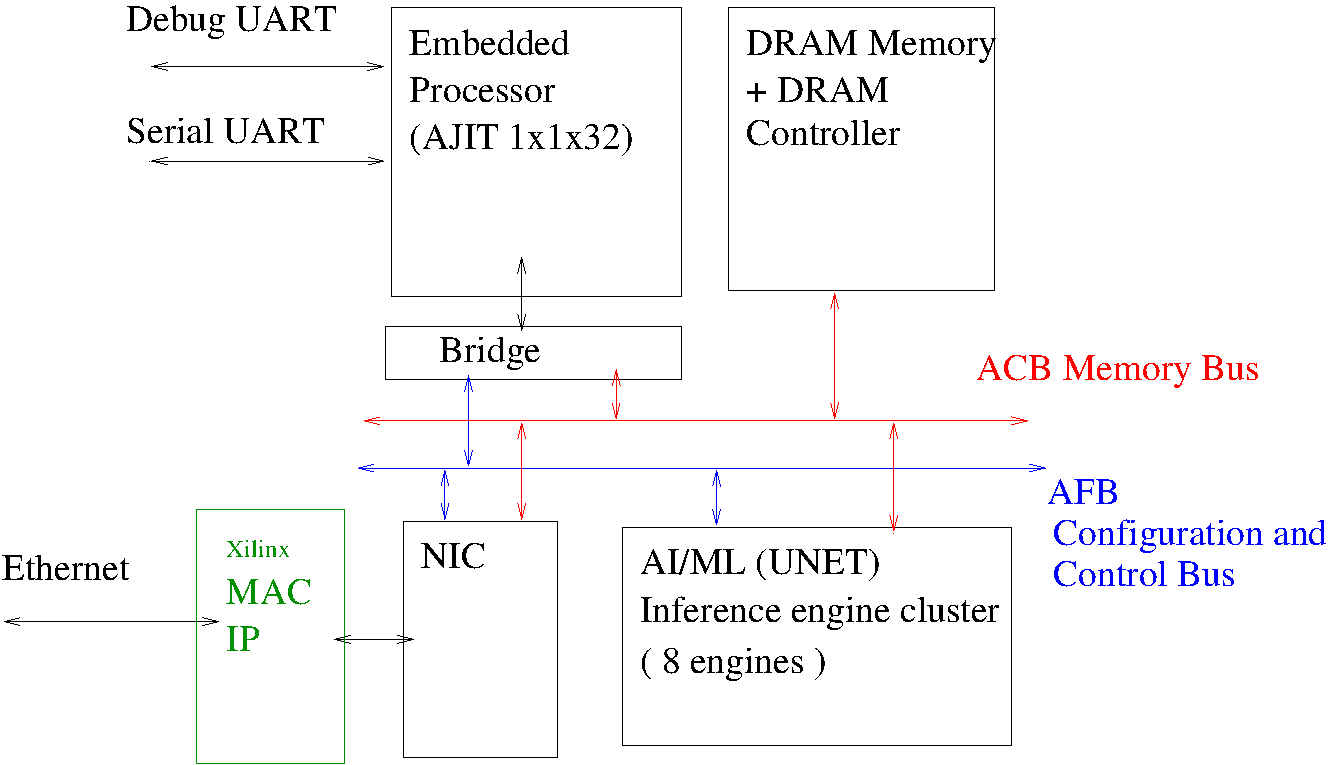
\includegraphics[width=\textwidth]{BlockDiagram.pdf}
	\caption{Block Diagram For SoC}
    \label{fig:SOC}
\end{figure}


\subsection{Processor Code}


\begin{algorithm}
	\caption{Pseudocode for processor code}
	\label{Algo:ProcessorCode}
	\begin{algorithmic}[1]
\State initialiseMemorySpaces()
\State initialiseNicQueues()
\State fetchKernelsThroughEthernet()

		\While {1}
\State	fetchInputsThroughEthernet()
	
\State	initliaseAcceleratorStates()
	
		\While {all accelerators not done}
		\For {engine in list\_of\_engines}
			\State convolve(engine,stage)
			\State updateState(engine,stage)
		\EndFor
	\EndWhile
	\State sendOutputsThroughEthernet()
\EndWhile
	\end{algorithmic}
\end{algorithm}
\begin{comment}
\begin{Verbatim}[numbers=left]
initialiseMemorySpaces()
initialiseNicQueues()
fetchKernelsThroughEthernet()

while(1) do
	fetchInputsThroughEthernet()
	
	initliaseAcceleratorStates()
	
	while (all accelerators not done) do
		for engine in list_of_engines do
			convolve(engine,stage)
			updateState(engine,stage)
		end for
	end while
	sendOutputsThroughEthernet()
end while
\end{Verbatim}
\end{comment}

Algorithm~\ref{Algo:ProcessorCode} explains the working of the processor code. It first initialise memory spaces required by all modules. These include the queues required by NIC, the kernel addresses for the accelerators and the memory spaces for receiving and storing tensors during computation by the engines. After the memory spaces are initialised, all the queues for NIC are configured and initialised, and the Network Interface Controller starts executing. The kernels are then fetched in through Ethernet, which is then followed by the input tensors for all the engines. With the setup ready, NIC is turned off and the engines are allowed to execute on the data stage by stage. When all the acclerators are done with their computation, the output data is sent to the host PC through Ethernet, where the output is verified for correctness.


The above is a simplified driver to demonstrate the functionality of using multiple accelerator engines inside the system using polling. The processor and the  accelerators both support the use of interrupts. The Interrupt Service Routine corresponding to the accelerator interrupts can be suitably confiured to allow the processor to be used for other processes, while the engines work on the compute-intensive AI/ML tasks, the completion of which can be signalled to the processor, at which the processor interrupts and schedules the next task to the accelerator before resuming its own execution.



\section{Processor NIC Interface}

The processor initializes the queues for the NIC and starts the NIC. When NIC receives data from MAC, it pops the free queue, which has empty packet buffers address stored in it, and writes the packet to that buffer. After successfully writing the packet, NIC pushes the address of the buffer to the rx queue; any buffer address in the rx queue indicates that this is the received packet and needs some action by the processor. While this thing is going on processor keeps polling the RX queue; as soon as it gets any data over there, it reads it and makes a decision. In this setup, processor is expected to store the packet at some memory location which is shared with the accelerator through its registers. After this packet storage is, complete processor pushes this address to the tx queue, which works as acknowledgment for the host; after receiving it, it(the host) sends the new packet. This is the overall flow for storing files in the memory.


Now to send the file out on the ethernet interface processor breaks the file into a number of packets, pops free queue for empty buffer address and stores packet at that address packet successfully processor pushes the buffer address to tx queue. The transmit engine running inside NIC which is polling this tx queue reads that buffer and sends it out. One by one all the packets sent out.



\section{Processor Accelerator Interface}

The processor begins by feeding the data to the registers 1 to 12. After that, it sets the bits 0 and 2 of register 0, which signals the accelerator to start working. The processor can then continue with other tasks or poll on the register 0 as it waits for the accelerator to complete, which is indicated by setting bit 3 of register 0 as high. Then, the processor updates the registers to the parameters for the next stage or image.


In addition, the accelerator has a control daemon which resets the registers, reads the data from the AFB\_ACCELERATOR\_REQUEST, writes them onto the accelerator registers, and sends back the response to the AFB\_ACCELERATOR\_RESPONSE. The control daemon runs infinitely waiting on AFB\_ACCELERATOR\_REQUEST requests from the processor.


The accelerator also has a worker daemon, which waits for the appropriate bits to be set in the r0 register. When the processor sends the request to execute through the registers, it calls the core function with the parameters stored by the processor in other registers. When the execution is completed, it writes back 0 into bit 3 of r0, thereby signaling the processor that the computation is completed.


The accelerator also has an interrupt daemon that waits on bit 4 of r0 and sets the signal ACCELERATOR\_INTERRUPT\_8 corresponding to the above bit. The interrupt signal is not currently used but can be utilised to prevent the processor from polling on r0 while the accelerator performs the computation.



\section{Scaling The Number Of Engines}\label{sec:scale_eng}

In Chapter~\ref{ch:3}, we described how the engine can exploit data-level parallelism to obtain higher throughput. In this section, we characterize the throughput improvement obtained by exploiting the parallelism between different images by implementing multiple accelerator engines in a single cluster, each working on its own input image. The number of engines actively running was increased from one to eight, and the following results were obtained:


\begin{table}
	\resizebox{\textwidth}{!}
	{
		\centering

		\begin{tabular}{P{0.16\linewidth} P{0.22\linewidth} P{0.22\linewidth} P{0.16\linewidth} P{0.16\linewidth} P{0.12\linewidth}}
		\toprule
			No. of active cores & 	Total time taken (*$10^6$ clock cycles)  &	Time per image (*$10^6$ clock cycles)	& Utilisation (normalised with one engine)  & Speedup (normalised with one engine) & Performance ( GOPS (fps) )\\

\toprule
			1 & 116.7 & 116.65 & 1 & 1 & 69(1.08)\\
\midrule
			2 & 119.7 & 59.85 & 0.97 & 1.94 & 134(2.09)\\
\midrule
			3 & 123.9 & 41.30 & 0.94 & 2.82 & 194(3.03)\\
\midrule
			4 & 133.4 & 33.35 & 0.87 & 3.48 & 240(3.75)\\
\midrule
			5 & 146.1 & 29.22 & 0.80 & 4.00 & 274(4.28)\\
\midrule
			6 & 162.2 & 27.04 & 0.72 & 4.32 & 296(4.63)\\
\midrule
			7 & 178.9 & 25.55 & 0.65 & 4.55 & 313(4.89)\\
\midrule
			8 & 201.2 & 25.15 & 0.58 & 4.64 & 318(4.97)\\
%1 & 93,249,712  & 93.25 & 1 & 1\\
%2 & 95,992,518  & 48.00 & 0.97 & 1.94\\
%3 & 99,271,600  & 33.09 & 0.94 & 2.82\\
%4 & 106,323,270  & 26.58 & 0.87 & 3.48\\
%5 & 116,061,718  & 23.21 & 0.80 & 4.00\\
%6 & 129,573,610  & 21.59 & 0.72 & 4.32\\
%7 & 144,883,176  & 20.69 & 0.64 & 4.47\\
%8 & 159,762,229  & 19.97 & 0.58 & 4.64\\
		\bottomrule
		\end{tabular}
	}
	\caption{Characterization of the performance of inference engine cluster}
	\label{tab:scale}
\end{table}

From the data, it is evident that we can efficiently scale the system to support 5 accelerator engines running in parallel without significant loss of performance. The performance degradation stems primarily from the use of a shared ACB connection to the memory, thereby causing contention for the resource. The degradation is small for up to 5 accelerators because the memory is being utilised around 10\% of the time, as seen in Table~\ref{tab:stage}. However, beyond 5 systems, the link becomes the bottleneck leading to greater performance degradation.


The primary reason for the degradation is the use of limited memory bandwidth, which is being multiplexed by all the engines, which gets intensified due to the high latency of DRAM accesses. To mitigate the issues, we have to reduce either the memory latency or improve the memory bandwidth, as seen by the engines. The first one can be obtained by using a cache, which can reduce the latency not only for kernels that are being shared by all the modules, but also the tensors which are accessed serially and benefit from the being loaded from the memory beforehand.


To address the more significant issue of limited memory bandwidth, we need a better memory management scheme and a network-on-chip that can provide high data rates to each of the engines when executed in the cluster. One solution is to execute the engines in a lock-step manner, where all the engines are synchronised to generate the same request simultaneously, and the request is supplied by a larger ported memory, which improves the bandwidth manifold. The disadvantage of such a technique is that it needs the engines to be synchronised, thereby needing them to be executed simultaneously.


\begin{comment}
\chapter{Demo Application}

When used as a standalone module, the accelerator can be accessed through following call in C:

void convolutionAll (uint16\_t rb, uint16\_t cb, uint16\_t rt, uint16\_t ct, uint16\_t chl\_out, uint16\_t chl\_in, uint16\_t rk, uint16\_t ck, uint32\_t index\_in1, uint32\_t index\_in2, uint32\_t index\_k, uint32\_t index\_out, uint32\_t scale\_val, uint16\_t shift\_val,uint16\_t pad, uint8\_t pool, uint8\_t concat uint8\_t activation);

When integrated with the processor, these values are acessed through registers as described in the chapter before. We demonstrate the results when the system was run with NIC and the processor, as follows:

\chapter{Other Ideas Tried}

Some other schemes were tried on the implementation. They are listed as follows:

\section{Prefetching of kernels}

In order to speed up the computation by reducing memory access during the stage, the kernels were pre-fetched during the execution of the previous stage. This was done using an independent daemon module which fetches the next layers kernels and writes them into the kernel pipes.


Prefetching of kernels led to a marginal performance improvement of \%, without any increase in the logic overhead.


Prefetching is not a default setting for the system. In order to implement pre-fetching, the user should make some modifications to the design - the call to kernel and/or input modules should be commented in the main convolution code, and run separately in a module ahead of the actual call to the convolution module. While doing so, the user should ensure that the pre-fetching module is executed in the sequential order of the layers to be computed, else it will lead to incorrect results.

\section{Cascading of convolution modules}

A three-module cascade was proposed as shown in the **fig**. Depending on the instruction, the modules can be configured in the following ways:

\begin{itemize}
\item Each module can run independently using the same input, with the kernels partitioned into each of the unit. This configuration is useful when the kernel size is very large, and kernel partitioning is required, thereby reducing the memory bandwidth requirements of fetching the inputs multiple times.
\item Alternatively, the modules can share the kernels, but work with different inputs.
\item Another configuration is to place two modules to work simulatneously on the first layer, with the third module working on the next layer. This not only allows to compute two layers simultaneously, but also reduces the need to store and load from memory after every layer. This configuration is efficient when the number of MAC operations of the second layer in the cascade is half of that of the first.
\item Similarly, the modules can be configured to have one module to work on first layer, the output of which are divided amongst the other two modules to work simulatneously for the second layer. This also allows to compute two layers simultaneously with reduced  memory bandwidth requirements for every layer. This configuration is efficient when the number of MAC operations of the first layer in the cascade is half of that of the second.
\item A three-layer cascade where the output of the first module is forwarded as input to the second, whose output is forwarded to the third, which is eventually written. This configuration is useful for networks with layers having a series of layers having identical number of computation.
\end{itemize}

\section{Quantization aware training}

In order to validate the correctness of the design, a software model was generated and trained on Tensorflow using quantization-aware methods. However, the losses for the chosen hyperparameters were not satisfactory, and required in-depth analysis into the training of the system. Hence, the validation of the hardware using real images was declared to be out of scope for the project.

\section{Sparsity}
	
UNET has a reLU layer after every convolution layer, and 3 transpose convolution layers. These layers create a lot of zeros as input for the convolution module (approximately 50\% and 75\% of the entries respectively), resulting in a very sparse matrix. This can be exploited to reduce the resource consumption by conditionally scheduling multiple MAC operations on one processing element. For example, if 4 MAC operations are tied to a single multiplier, then, in expectation, the latency (in clock cycles) will be $\dfrac{1}{16} + \dfrac{4*1}{16} + \dfrac{6*2}{16} + \dfrac{4*3}{16} + \dfrac{1*4}{16} = \dfrac{33}{16} \approx 2$. Thus, by using the same number of MAC units, we can improve performance by 48\% for layers preceded by reLU. For transpose convolution, the performance improves by 305\%. However, as the distribution of non-zero data is not equal across all processing elements, some elements will execute faster than others. Thus, in order to achieve the performance benefits described above, it will be necessary to individually buffer inputs and kernels for each processing element, letting the processing elements can work independently of each other without stalling the pipeline. Not only this, we need additional control logic at the accumulation and postprocessing modules to facilitate the uneven timing of each processing element. The overhead generated by such a scheme is very likely to outweigh the benefits, and hence, was not implemented.

\end{comment}

\chapter{Summary}

In this work, we present a hardware acceleration engine for AI/ML inference tasks. The engine is algorithmically designed using the AHIR-V2 tools, and is optimised for maximum compute-to-memory ratio using minimal on-chip buffers. We demonstrate an application of the engine by developing a image segmentation pipeline on UNET, a well-known architecture for image segmentation. We obtain an average throughput of 85 GOPS, with the peak throughput of a stage matching the theoretical peak performance of 96 GOPS when run on a single engine with an average compute-to-memory ratio of 873 operations/byte (OPB).

We also integrate the engine with the AJIT processor and Network Interface Controller (NIC) to generate a system on chip (SoC) capable of performing at-edge AI/ML inference tasks. Using the SoC, we establish the correctness of the acceleration engine using a testbench to validate the output sent to the host machine after every stage. We further show that the engine architecture scales well on replication, attaining an average performance of over 240 GOPS when employing the four engines simultaneously, with an average utilisation in excess of 62\% over the duration of the computation, with an image throughput of over 3.5fps, which increases to 5fps for eight engine cluster. We also compare our engine with other works from reported literature, and find our engine to be competitive in terms of its resource efficiency.


Through our examination of the characteristics of the engine, we find that we could add some changes to improve performance and robustness further. These optimizations are listed as future work here:

\begin{itemize}
	\item The critical bottleneck when scaling to a large cluster is the memory bandwidth. Thus, utilising an improved memory subsystem with a global cache can provide a higher memory bandwidth to cater to the high data IO rates needed for the accelerator engine clusters.
	\item Another area of optimization is the use of the large multiplier width of the DSP slices (27x18) in Xilinx FPGAs to efficiently compute two 8-bit MACs simultaneously using one DSP slice.
	\item By providing support for computation on 16-bit quantised data and writeback of 32-bit output to allow for preventing quantisation losses at critical layers, we can provide better flexibility to the user to balance inference accuracy and performance requirements.
\end{itemize}





\begin{comment}
\chapter{Future Work}

The following tasks are to be done as part of Stage 2 requirements:

\begin{enumerate}
    \item Perform verification of the synthesized end-to-end design with real image data, and measure appropriate parameters like Intersection Over Union (IOU) and accuracy to quantify the degradation due to the use of fixed-point representation
    % \item Since concatenation and transpose convolution module just change the input format, employ them as a specialized input module for convolution instead of performing an end-to-end memory operation
    \item Hiding memory fetch latency by pre-fetching next kernel and inputs during execution of the previous convolution
    \item Move to 150MHz by shortening the critical paths (combinational logic) through addition of appropriate buffers, doubling the raw performance of the system
    \item Utilize sparsity by dividing work of multiple units into 1 multiplier. By using one multiplier for 4 units, we get a reduction in core resource consumption by 4x, for an expected performance degradation of 51\% during normal convolution, and 24\% for transpose convolution, improving resource efficiency by 92\% and 204\% respectively. Assuming small overhead, this modification can help us achieve the goal of 2 GOPS/KLUT without incorporating other modification discussed in this chapter
    \item Explore cascading of multiple calls to the convolution module to reduce memory dependence and improve performance
    \item Develop a scheme to efficiently scale the design to achieve high throughput in terms of frames processed per second
\end{enumerate}
\end{comment}

% \begin{thebibliography}{00}


% \bibitem{doppler_bth}\href{https://ieeexplore.ieee.org/stamp/stamp.jsp?tp=&arnumber=1057560}{J. Marcum, "A statistical theory of target detection by pulsed radar," in IRE Transactions on Information Theory, vol. 6, no. 2, pp. 59-267, April 1960, doi: 10.1109/TIT.1960.1057560.}

% \end{thebibliography}

\bibliographystyle{ieeetr}
\bibliography{thesisTemplate}{}
\end{document}



% \section{Concatenation}

% This module performs concatenation of two tensors along the channel. Since the data is stored in column-major form, concatenation along channels involves reading alternately from the two modules, and sending the data to the output.
% \\

% The module keeps a track of two counters for the channels - one for the input side and one for the output. The first counter indicates the number of input channels left, and on reset, it switches input from the first tensor to the second. This interleaving results in the concatenation of the two tensors. The second counter maintains the count of the output channels, which is the sum of the input channels. On reset, this counter is used to change the row and column for the next input.
% \\

% Since concatenation occurs only during the decoding loop, it has inputs and output which have channels that are multiples of 8. This permits the module to read whole words from the memory at a given point in time and send it as it is as the output. Hence, the module is optimised to directly forward whole words from one memory address to another.
% \\

% It should be noted that the operation of the module is totally memory intensive, with no computation.


% \section{Transpose convolution}

% Transpose convolution involves three steps:

% \begin{enumerate}
%     \item Writing the tensor with zeros at appropriate spacing
%     \item Depadding the extra layers in the tensor
%     \item Performing convolution operation on the resultant tensor
% \end{enumerate}

% The deconvolution module designed here does the first two steps, as the third step can be done by a direct call to the convolution module. Furthermore, to optimize the performance, the two steps are done simultaneously by performing depadding by not padding with zeros at locations which will eventually get depadded. The padding and depadding happens by addition of zeros at the appropriate rows and between adjacent columns.
% \\

% Again, like the concatenation module, number of channels for the tensors are multiples of 8, and hence, the start of each row and column is word-aligned with the memory. Hence, it suffices for the module to write the output data directly into the memory without intermediate processing, leading in a full-rate execution of the module (1 memory operation every clock cycle).
% \\

% Transpose convolution module also has no convolution, and its performance depends on the memory bandwidth and latency available.


